\subsection{The Bayesian Framework}
Bayesian inference is a layered process. For classification the modified primal problem,
\begin{align}
\min\limits_{w,b,e_c} J_p (w,e_c) = \mu \frac{1}{2}\mathbf{w}^T\mathbf{w} + \zeta \frac{1}{2} \sum\limits_{k = 1}^{N} e^2_{c,k} \\
\text{such that } y_k [\mathbf{w}^T \varphi(\mathbf{x}_k) + b] = 1 - e_{c,k}, k = 1, \dots, N 
\end{align}
is used which eventually leads to the dual space classifier\footnote{Support Vector Machines: Methods and Applications, Suykens et al., page 119}
\begin{align}
y(x) = \text{sign}[\frac{1}{\mu} \sum\limits_{k=1}^{N}\alpha_k K(x,x_k) + b]
\end{align} 
It follows that the primal weight space parameters $w,b$ the hyper-parameters $\mu,\zeta$ and finally the kernel parameters (if any) have to be determined. The hyper-parameters $\mu,\zeta$ are a different way to express $\gamma$, which was used in previous formulations. The relation $\gamma = \frac{\zeta}{\mu}$ holds \footnote{Support Vector Machines: Methods and Applications, Suykens et al., page 118}, which can be checked by substituting $\mu = 1$.
The unknowns will be found following a three layered process. The first layer focuses on the weight vector and the bias terms defining $\mathcal{D} = \{x_k,y_k\}^N_{k = 1}$ and using $\mathcal{H}_{i}$ to denote different models i.e. radial basis function kernels with different width. The first level uses the equation:\footnote{Support Vector Machines: Methods and Applications, Suykens et al., page 122}
\begin{equation}
p(\mathbf{w},b|\mathcal{D},\mu,\zeta,\mathcal{H}_\sigma) = \frac{p(\mathcal{D}|\mathbf{w},b,\mu,\zeta,\mathcal{H}_\sigma)}{p(\mathcal{D}|\mu,\zeta,\mathcal{H}_\sigma)} p(\mathbf{w},b|\mu,\zeta,\mathcal{H}_\sigma)
\end{equation}
With $p(\mathcal{D}|\mu,\zeta,\mathcal{H}_\sigma)$ denoting the evidence which is determined by integrating over all possible values of $\mathbf{w},b$ and normalizing the result. $\mathbf{w},b$ follow from the first level, which is then used in the second layer to find $\mu$ and $\zeta$ by maximizing:
\begin{equation}
p(\mu,\zeta|\mathcal{D},\mathcal{H}_\sigma) = \frac{p(\mathcal{D}|\mu,\zeta,\mathcal{H}_\sigma)}{p(\mathcal{D}|\mathcal{H}_\sigma)} p(\mu,\zeta|\mathcal{H}_\sigma). 
\end{equation}
Which leads to the lowest third level where the kernel parameters are found:
\begin{equation}
p(\mathcal{H}_\sigma|\mathcal{D}) = \frac{p(\mathcal{D}|\mathcal{H}_\sigma)}{p(\mathcal{D})} p(\mathcal{H}_\sigma).
\end{equation}
For function estimation the picture is similar, but a couple of small modifications have to be made. For example assuming a hyper-parameter vector $\zeta_{1\dots N} = [\zeta_1,\dots,\zeta_N]$.
Using Bayesian inference also makes it possible to compute error bounds. The model found from the initial parameters $\sigma^2 = 0.01$, $\gamma = 10$ is shown in figure~\ref{fig:bayesianInf}. It is not perfect but all training points lie indeed inside the confidence interval. Choosing an initial point closer to the global optimum will probably results in better parameters $\sigma$ and $\gamma$. \\
A good example for binary classification is the simplified iris data set. Using bayesian inference the posterior class probabilities can be estimated. This has been done for a classifier trained using $\gamma = 5$ and $\sigma^2 = 0.75$. The result is shown in figure~\ref{fig:bayesianClass}. The purple indicates that the classifier will place points in this area in the positive class, while data in the blue area will be placed in the negative class. Like it was observed earlier the regularization parameter reduces model complexity for low values and stresses good fit to the data for high values. The kernel density on the other hand stresses fit for small values and model complexity reduction for larger widths. \\
\begin{figure}
\centering
\includegraphics[width=0.25\linewidth]{../src/figure/bayesianInf}
\caption{Bayesian inference schematic.}
\label{fig:bayesianInf}
\end{figure}
\begin{figure}
\centering
%% This file was created by matlab2tikz.
% Minimal pgfplots version: 1.3
%
%The latest updates can be retrieved from
%  http://www.mathworks.com/matlabcentral/fileexchange/22022-matlab2tikz
%where you can also make suggestions and rate matlab2tikz.
%
\documentclass[tikz]{standalone}
\usepackage{pgfplots}
\usepackage{grffile}
\pgfplotsset{compat=newest}
\usetikzlibrary{plotmarks}
\usepackage{amsmath}

\begin{document}
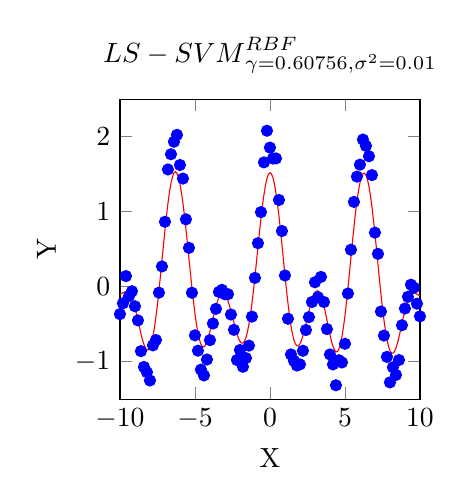
\begin{tikzpicture}

\begin{axis}[%
width=1.5in,
height=1.5in,
scale only axis,
xmin=-10,
xmax=10,
xlabel={X},
ymin=-1.5,
ymax=2.5,
ylabel={Y},
title style={font=\bfseries},
title={$\text{LS-SVM}_{\gamma\text{=0.60756,}\sigma{}^\text{2}\text{=0.01}}^{\text{RBF}}$}
]
\addplot [color=red,solid,forget plot]
  table[row sep=crcr]{%
-10	-0.103034596060459\\
-9.9	-0.0924077535053527\\
-9.8	-0.0810321511775389\\
-9.7	-0.0715324776926961\\
-9.6	-0.0669422274212075\\
-9.5	-0.0703889602254681\\
-9.4	-0.0847327830654409\\
-9.3	-0.112203880139092\\
-9.2	-0.154085056276393\\
-9.1	-0.210478528933273\\
-9	-0.280184436179667\\
-8.9	-0.360704025474425\\
-8.8	-0.448365465221515\\
-8.7	-0.538556502394305\\
-8.6	-0.626037168250545\\
-8.5	-0.705298457717249\\
-8.4	-0.770930122889762\\
-8.3	-0.817962781891637\\
-8.2	-0.84215621128021\\
-8.1	-0.840215941068152\\
-8	-0.809932284871487\\
-7.9	-0.750247348987414\\
-7.8	-0.661263982454023\\
-7.7	-0.544214284038502\\
-7.6	-0.401403584146788\\
-7.5	-0.236139637102408\\
-7.4	-0.0526482594857303\\
-7.3	0.144031275392607\\
-7.2	0.348182358878664\\
-7.1	0.553589404784394\\
-7	0.753763257072639\\
-6.9	0.942208657883996\\
-6.8	1.1127178173584\\
-6.7	1.25966517842964\\
-6.6	1.37827423187069\\
-6.5	1.46482911056944\\
-6.4	1.51681140218854\\
-6.3	1.53295432896495\\
-6.2	1.51321930610937\\
-6.1	1.4587108511435\\
-6	1.37155241882695\\
-5.9	1.25474671874462\\
-5.8	1.11203962166202\\
-5.7	0.947798384554648\\
-5.6	0.766905007343529\\
-5.5	0.574656702419758\\
-5.4	0.376659917946314\\
-5.3	0.178703377681614\\
-5.2	-0.0134007341154479\\
-5.1	-0.194011042277\\
-5	-0.357881239848352\\
-4.9	-0.500400101754449\\
-4.8	-0.617826402457124\\
-4.7	-0.707494693438359\\
-4.6	-0.767968638016936\\
-4.5	-0.799123065023287\\
-4.4	-0.802143297779957\\
-4.3	-0.779439459408219\\
-4.2	-0.734482960864626\\
-4.1	-0.671580819994145\\
-4	-0.595609560783958\\
-3.9	-0.511733273203496\\
-3.8	-0.425129590914951\\
-3.7	-0.340743154928029\\
-3.6	-0.263079532980724\\
-3.5	-0.196045010775177\\
-3.4	-0.142830791771985\\
-3.3	-0.105835347689468\\
-3.2	-0.0866167825776274\\
-3.1	-0.0858681383990343\\
-3	-0.103411799648806\\
-2.9	-0.138213183396576\\
-2.8	-0.188417183727886\\
-2.7	-0.251412127445675\\
-2.6	-0.323924742251484\\
-2.5	-0.402146177592433\\
-2.4	-0.481884567230999\\
-2.3	-0.558735486453836\\
-2.2	-0.628259294532108\\
-2.1	-0.686154491102442\\
-2	-0.728418701089652\\
-1.9	-0.751492793960255\\
-1.8	-0.752387585816612\\
-1.7	-0.728795304214125\\
-1.6	-0.679188756073778\\
-1.5	-0.602909842564045\\
-1.4	-0.500246201809438\\
-1.3	-0.372491139137642\\
-1.2	-0.221978495108584\\
-1.1	-0.052081502049025\\
-1	0.132836285597705\\
-0.9	0.327528560621392\\
-0.799999999999999	0.526038727981508\\
-0.699999999999999	0.721936525498598\\
-0.6	0.908608605488591\\
-0.5	1.0795827284767\\
-0.399999999999999	1.22885682292373\\
-0.299999999999999	1.35120020298932\\
-0.199999999999999	1.4423966655644\\
-0.0999999999999996	1.49940832069644\\
0	1.52045305269972\\
0.0999999999999996	1.50500385912029\\
0.199999999999999	1.45373061015538\\
0.299999999999999	1.36841036215803\\
0.399999999999999	1.25182963773846\\
0.5	1.10769214520262\\
0.6	0.940531750979476\\
0.699999999999999	0.755617886760161\\
0.799999999999999	0.558833364158772\\
0.9	0.356505371753253\\
1	0.155179210542487\\
1.1	-0.0386614861826507\\
1.2	-0.218908916525321\\
1.3	-0.380148434224328\\
1.4	-0.517942423702936\\
1.5	-0.629046830731622\\
1.6	-0.711536402668681\\
1.7	-0.764829181544373\\
1.8	-0.789616217000695\\
1.9	-0.787715370276717\\
2	-0.761876033398643\\
2.1	-0.71556362783275\\
2.2	-0.652749348412112\\
2.3	-0.577723286144426\\
2.4	-0.494939768500007\\
2.5	-0.40889442981833\\
2.6	-0.32402475035394\\
2.7	-0.244620714025637\\
2.8	-0.174730540328445\\
2.9	-0.118048451730617\\
3	-0.0777769926130666\\
3.1	-0.0564647824268098\\
3.2	-0.0558303446912548\\
3.3	-0.0765917735502247\\
3.4	-0.11832817196698\\
3.5	-0.17940001239501\\
3.6	-0.256950794563972\\
3.7	-0.347002052310924\\
3.8	-0.444639935115007\\
3.9	-0.544277482232278\\
4	-0.639965834541782\\
4.1	-0.725722709520112\\
4.2	-0.795848493649644\\
4.3	-0.845208157327731\\
4.4	-0.869467939170201\\
4.5	-0.865285619254506\\
4.6	-0.830458932443032\\
4.7	-0.764036674916607\\
4.8	-0.666392044551242\\
4.9	-0.539250529145403\\
5	-0.385659082032698\\
5.1	-0.209882859794184\\
5.2	-0.0172220993075777\\
5.3	0.186246133485757\\
5.4	0.39398190244768\\
5.5	0.599320068269959\\
5.6	0.795793541292616\\
5.7	0.977406814282306\\
5.8	1.13883590885616\\
5.9	1.27554785217494\\
6	1.38385047631223\\
6.1	1.46089666147675\\
6.2	1.50467250401068\\
6.3	1.51399516262758\\
6.4	1.4885349389801\\
6.5	1.4288611929483\\
6.6	1.33649754501469\\
6.7	1.21396250256155\\
6.8	1.06476954056722\\
6.9	0.893365980521173\\
7	0.705000940388274\\
7.1	0.505526045091972\\
7.2	0.301145001612354\\
7.3	0.0981366385861365\\
7.4	-0.0974210899512405\\
7.5	-0.279901496523124\\
7.6	-0.44433669594411\\
7.7	-0.586574750115089\\
7.8	-0.703388355625166\\
7.9	-0.792543889162952\\
8	-0.852842344876384\\
8.1	-0.884141786475728\\
8.2	-0.887365137810447\\
8.3	-0.864489244586956\\
8.4	-0.818503602283442\\
8.5	-0.753322477764944\\
8.6	-0.673634309611475\\
8.7	-0.584678112789672\\
8.8	-0.491947601709095\\
8.9	-0.400837982134765\\
9	-0.316264938807604\\
9.1	-0.242296947627253\\
9.2	-0.181847661369015\\
9.3	-0.136472732245758\\
9.4	-0.106304515298641\\
9.5	-0.0901398621260733\\
9.6	-0.0856735506877209\\
9.7	-0.0898469160242713\\
9.8	-0.0992625096179794\\
9.9	-0.110605131753092\\
10	-0.12100980525799\\
};
\addplot [color=blue,only marks,mark=*,mark options={solid},forget plot]
  table[row sep=crcr]{%
-10	-0.365928104442444\\
-9.8	-0.221446760756492\\
-9.6	0.141410542499974\\
-9.4	-0.127039811490799\\
-9.2	-0.0607138156567727\\
-9	-0.260997520295833\\
-8.8	-0.449394746554925\\
-8.6	-0.859203591315005\\
-8.4	-1.07012983994485\\
-8.2	-1.14080160805147\\
-8	-1.25080480458164\\
-7.8	-0.782496567520973\\
-7.6	-0.7110732186952\\
-7.4	-0.079662037023974\\
-7.2	0.270013529372922\\
-7	0.865119219542747\\
-6.8	1.56298674574302\\
-6.6	1.76609238695701\\
-6.4	1.93246354665889\\
-6.2	2.0241791499525\\
-6	1.62255366381118\\
-5.8	1.44161033038666\\
-5.6	0.897878200648367\\
-5.4	0.517401436969264\\
-5.2	-0.0809103948519976\\
-5	-0.648358534013222\\
-4.8	-0.853218154708919\\
-4.6	-1.10597471690631\\
-4.4	-1.18293777979472\\
-4.2	-0.97106973419971\\
-4	-0.712546036242109\\
-3.8	-0.490908298165794\\
-3.6	-0.295521926402203\\
-3.4	-0.0703571750280591\\
-3.2	-0.0418632286505383\\
-3	-0.101517599304707\\
-2.8	-0.10033197630765\\
-2.6	-0.370950251734923\\
-2.4	-0.575144702187335\\
-2.2	-0.977595551284394\\
-2	-0.844492791705589\\
-1.8	-1.06793690834119\\
-1.6	-0.952261695397724\\
-1.4	-0.785873533027652\\
-1.2	-0.399188291966348\\
-1	0.11712276553897\\
-0.799999999999999	0.580011915626202\\
-0.6	0.994073603294988\\
-0.399999999999999	1.65739334562653\\
-0.199999999999999	2.07950855314113\\
0	1.85452035528\\
0.199999999999999	1.70926581476288\\
0.399999999999999	1.71026543774087\\
0.6	1.15626769919301\\
0.799999999999999	0.742271086071982\\
1	0.14959144820096\\
1.2	-0.427433600265483\\
1.4	-0.903373535168694\\
1.6	-0.988193527881448\\
1.8	-1.05126720871999\\
2	-1.0358512418469\\
2.2	-0.854423225944074\\
2.4	-0.577864924061717\\
2.6	-0.40553744933982\\
2.8	-0.204722209816492\\
3	0.0592801031257328\\
3.2	-0.13942934304599\\
3.4	0.130649240307429\\
3.6	-0.204340361786744\\
3.8	-0.565236267312748\\
4	-0.903797843066106\\
4.2	-1.03637731433893\\
4.4	-1.31428661987946\\
4.6	-0.980434312967732\\
4.8	-1.01015274903283\\
5	-0.761450533975107\\
5.2	-0.0908878968065172\\
5.4	0.492389657640184\\
5.6	1.13058589302983\\
5.8	1.46772989918675\\
6	1.6271839407589\\
6.2	1.96158561217912\\
6.4	1.87746936020765\\
6.6	1.73902687709014\\
6.8	1.48788957059651\\
7	0.720831805909899\\
7.2	0.437801905700275\\
7.4	-0.331067091401463\\
7.6	-0.651507149163496\\
7.8	-0.935911864891144\\
8	-1.27611825876353\\
8.2	-1.07487463249801\\
8.4	-1.17647767911817\\
8.6	-0.97799570674273\\
8.8	-0.513870240653853\\
9	-0.29102066772989\\
9.2	-0.134897568742019\\
9.4	0.0267707034103775\\
9.6	-0.0127903761230497\\
9.8	-0.226369203963368\\
10	-0.395044936133213\\
};
\end{axis}
\end{tikzpicture}%
\end{document}
% This file was created by matlab2tikz.
% Minimal pgfplots version: 1.3
%
%The latest updates can be retrieved from
%  http://www.mathworks.com/matlabcentral/fileexchange/22022-matlab2tikz
%where you can also make suggestions and rate matlab2tikz.
%
\documentclass[tikz]{standalone}
\usepackage{pgfplots}
\usepackage{grffile}
\pgfplotsset{compat=newest}
\usetikzlibrary{plotmarks}
\usepackage{amsmath}

\begin{document}
\definecolor{mycolor1}{rgb}{0.00000,0.44700,0.74100}%
\definecolor{mycolor2}{rgb}{0.85000,0.32500,0.09800}%
\definecolor{mycolor3}{rgb}{0.49400,0.18400,0.55600}%
%
\begin{tikzpicture}

\begin{axis}[%
width=4.5in,
height=1.5in,
scale only axis,
xmin=-10,
xmax=10,
xlabel={X},
ymin=-1.5,
ymax=2.5,
ylabel={Y},
title={$\text{LS-SVM}_{\gamma\text{=0.60756, }\sigma{}^\text{2}\text{=0.01}}^{\text{RBF}}\text{ and 95\% (2}\sigma\text{) bands}$},
axis x line*=bottom,
axis y line*=left
]
\addplot [color=mycolor1,solid,forget plot]
  table[row sep=crcr]{%
-10	-0.103034596060459\\
-9.8	-0.0810321511775389\\
-9.6	-0.0669422274212075\\
-9.4	-0.0847327830654409\\
-9.2	-0.154085056276393\\
-9	-0.280184436179667\\
-8.8	-0.448365465221515\\
-8.6	-0.626037168250545\\
-8.4	-0.770930122889762\\
-8.2	-0.84215621128021\\
-8	-0.809932284871487\\
-7.8	-0.661263982454023\\
-7.6	-0.401403584146788\\
-7.4	-0.0526482594857303\\
-7.2	0.348182358878664\\
-7	0.753763257072639\\
-6.8	1.1127178173584\\
-6.6	1.37827423187069\\
-6.4	1.51681140218854\\
-6.2	1.51321930610937\\
-6	1.37155241882695\\
-5.8	1.11203962166202\\
-5.6	0.766905007343529\\
-5.4	0.376659917946314\\
-5.2	-0.0134007341154479\\
-5	-0.357881239848352\\
-4.8	-0.617826402457124\\
-4.6	-0.767968638016936\\
-4.4	-0.802143297779957\\
-4.2	-0.734482960864626\\
-4	-0.595609560783958\\
-3.8	-0.425129590914951\\
-3.6	-0.263079532980724\\
-3.4	-0.142830791771985\\
-3.2	-0.0866167825776274\\
-3	-0.103411799648806\\
-2.8	-0.188417183727886\\
-2.6	-0.323924742251484\\
-2.4	-0.481884567230999\\
-2.2	-0.628259294532108\\
-2	-0.728418701089652\\
-1.8	-0.752387585816612\\
-1.6	-0.679188756073778\\
-1.4	-0.500246201809438\\
-1.2	-0.221978495108584\\
-1	0.132836285597705\\
-0.799999999999999	0.526038727981508\\
-0.6	0.908608605488591\\
-0.399999999999999	1.22885682292373\\
-0.199999999999999	1.4423966655644\\
0	1.52045305269972\\
0.199999999999999	1.45373061015538\\
0.399999999999999	1.25182963773846\\
0.6	0.940531750979476\\
0.799999999999999	0.558833364158772\\
1	0.155179210542487\\
1.2	-0.218908916525321\\
1.4	-0.517942423702936\\
1.6	-0.711536402668681\\
1.8	-0.789616217000695\\
2	-0.761876033398643\\
2.2	-0.652749348412112\\
2.4	-0.494939768500007\\
2.6	-0.32402475035394\\
2.8	-0.174730540328445\\
3	-0.0777769926130666\\
3.2	-0.0558303446912548\\
3.4	-0.11832817196698\\
3.6	-0.256950794563972\\
3.8	-0.444639935115007\\
4	-0.639965834541782\\
4.2	-0.795848493649644\\
4.4	-0.869467939170201\\
4.6	-0.830458932443032\\
4.8	-0.666392044551242\\
5	-0.385659082032698\\
5.2	-0.0172220993075777\\
5.4	0.39398190244768\\
5.6	0.795793541292616\\
5.8	1.13883590885616\\
6	1.38385047631223\\
6.2	1.50467250401068\\
6.4	1.4885349389801\\
6.6	1.33649754501469\\
6.8	1.06476954056722\\
7	0.705000940388274\\
7.2	0.301145001612354\\
7.4	-0.0974210899512405\\
7.6	-0.44433669594411\\
7.8	-0.703388355625166\\
8	-0.852842344876384\\
8.2	-0.887365137810447\\
8.4	-0.818503602283442\\
8.6	-0.673634309611475\\
8.8	-0.491947601709095\\
9	-0.316264938807604\\
9.2	-0.181847661369015\\
9.4	-0.106304515298641\\
9.6	-0.0856735506877209\\
9.8	-0.0992625096179794\\
10	-0.12100980525799\\
};
\addplot [color=mycolor2,dash pattern=on 1pt off 3pt on 3pt off 3pt,forget plot]
  table[row sep=crcr]{%
-10	0.165205967334523\\
-9.8	0.187208412217443\\
-9.6	0.201298335973774\\
-9.4	0.183507780329541\\
-9.2	0.114155507118589\\
-9	-0.0119438727846855\\
-8.8	-0.180124901826534\\
-8.6	-0.357796604855563\\
-8.4	-0.50268955949478\\
-8.2	-0.573915647885228\\
-8	-0.541691721476505\\
-7.8	-0.393023419059041\\
-7.6	-0.133163020751807\\
-7.4	0.215592303909251\\
-7.2	0.616422922273646\\
-7	1.02200382046762\\
-6.8	1.38095838075338\\
-6.6	1.64651479526567\\
-6.4	1.78505196558352\\
-6.2	1.78145986950435\\
-6	1.63979298222193\\
-5.8	1.380280185057\\
-5.6	1.03514557073851\\
-5.4	0.644900481341296\\
-5.2	0.254839829279534\\
-5	-0.0896406764533708\\
-4.8	-0.349585839062143\\
-4.6	-0.499728074621954\\
-4.4	-0.533902734384975\\
-4.2	-0.466242397469644\\
-4	-0.327368997388976\\
-3.8	-0.156889027519969\\
-3.6	0.00516103041425736\\
-3.4	0.125409771622997\\
-3.2	0.181623780817354\\
-3	0.164828763746176\\
-2.8	0.0798233796670955\\
-2.6	-0.0556841788565024\\
-2.4	-0.213644003836058\\
-2.2	-0.360018737521891\\
-2	-0.460198850560934\\
-1.8	-0.486046468747948\\
-1.6	-0.417866254742839\\
-1.4	-0.239698340587518\\
-1.2	0.0385651824123845\\
-1	0.393379962453168\\
-0.799999999999999	0.786582404834259\\
-0.6	1.16915228234176\\
-0.399999999999999	1.489400499777\\
-0.199999999999999	1.70294034241768\\
0	1.780996729553\\
0.199999999999999	1.71427428700867\\
0.399999999999999	1.51237331459174\\
0.6	1.20107542783264\\
0.799999999999999	0.819377041011523\\
1	0.41572288739795\\
1.2	0.0416347609956469\\
1.4	-0.257394562481016\\
1.6	-0.450213901337741\\
1.8	-0.523275099932031\\
2	-0.493656182869925\\
2.2	-0.384508791401894\\
2.4	-0.226699205105067\\
2.6	-0.055784186958958\\
2.8	0.093510023066537\\
3	0.190463570781915\\
3.2	0.212410218703727\\
3.4	0.149912391428001\\
3.6	0.0112897688310094\\
3.8	-0.176399371720025\\
4	-0.3717252711468\\
4.2	-0.527607930254662\\
4.4	-0.601227375775219\\
4.6	-0.56221836904805\\
4.8	-0.39815148115626\\
5	-0.117418518637717\\
5.2	0.251018464087404\\
5.4	0.662222465842662\\
5.6	1.0640341046876\\
5.8	1.40707647225114\\
6	1.65209103970721\\
6.2	1.77291306740566\\
6.4	1.75677550237508\\
6.6	1.60473810840968\\
6.8	1.3330101039622\\
7	0.973241503783256\\
7.2	0.569385565007335\\
7.4	0.170819473443741\\
7.6	-0.176096132549128\\
7.8	-0.435147792230185\\
8	-0.584601781481402\\
8.2	-0.619124574415465\\
8.4	-0.55026303888846\\
8.6	-0.405393746216493\\
8.8	-0.223707038314113\\
9	-0.0480243754126228\\
9.2	0.0863929020259662\\
9.4	0.161936048096341\\
9.6	0.182567012707261\\
9.8	0.168978053777002\\
10	0.147230758136992\\
};
\addplot [color=mycolor2,dash pattern=on 1pt off 3pt on 3pt off 3pt,forget plot]
  table[row sep=crcr]{%
-10	-0.371275159455441\\
-9.8	-0.349272714572521\\
-9.6	-0.335182790816189\\
-9.4	-0.352973346460423\\
-9.2	-0.422325619671374\\
-9	-0.548424999574649\\
-8.8	-0.716606028616497\\
-8.6	-0.894277731645527\\
-8.4	-1.03917068628474\\
-8.2	-1.11039677467519\\
-8	-1.07817284826647\\
-7.8	-0.929504545849005\\
-7.6	-0.66964414754177\\
-7.4	-0.320888822880712\\
-7.2	0.0799417954836825\\
-7	0.485522693677658\\
-6.8	0.844477253963419\\
-6.6	1.11003366847571\\
-6.4	1.24857083879356\\
-6.2	1.24497874271439\\
-6	1.10331185543197\\
-5.8	0.843799058267035\\
-5.6	0.498664443948547\\
-5.4	0.108419354551333\\
-5.2	-0.28164129751043\\
-5	-0.626121803243334\\
-4.8	-0.886066965852106\\
-4.6	-1.03620920141192\\
-4.4	-1.07038386117494\\
-4.2	-1.00272352425961\\
-4	-0.863850124178939\\
-3.8	-0.693370154309933\\
-3.6	-0.531320096375706\\
-3.4	-0.411071355166967\\
-3.2	-0.354857345972609\\
-3	-0.371652363043787\\
-2.8	-0.456657747122868\\
-2.6	-0.592165305646466\\
-2.4	-0.750125130625939\\
-2.2	-0.896499851542326\\
-2	-0.99663855161837\\
-1.8	-1.01872870288528\\
-1.6	-0.940511257404718\\
-1.4	-0.760794063031357\\
-1.2	-0.482522172629552\\
-1	-0.127707391257758\\
-0.799999999999999	0.265495051128758\\
-0.6	0.648064928635423\\
-0.399999999999999	0.968313146070456\\
-0.199999999999999	1.18185298871111\\
0	1.25990937584644\\
0.199999999999999	1.1931869333021\\
0.399999999999999	0.991285960885189\\
0.6	0.679988074126308\\
0.799999999999999	0.298289687306022\\
1	-0.105364466312976\\
1.2	-0.479452594046289\\
1.4	-0.778490284924855\\
1.6	-0.97285890399962\\
1.8	-1.05595733406936\\
2	-1.03009588392736\\
2.2	-0.920989905422329\\
2.4	-0.763180331894948\\
2.6	-0.592265313748921\\
2.8	-0.442971103723426\\
3	-0.346017556008048\\
3.2	-0.324070908086236\\
3.4	-0.386568735361962\\
3.6	-0.525191357958954\\
3.8	-0.712880498509988\\
4	-0.908206397936764\\
4.2	-1.06408905704463\\
4.4	-1.13770850256518\\
4.6	-1.09869949583801\\
4.8	-0.934632607946224\\
5	-0.65389964542768\\
5.2	-0.285462662702559\\
5.4	0.125741339052699\\
5.6	0.527552977897634\\
5.8	0.870595345461177\\
6	1.11560991291725\\
6.2	1.2364319406157\\
6.4	1.22029437558512\\
6.6	1.06825698161971\\
6.8	0.79652897717224\\
7	0.436760376993293\\
7.2	0.032904438217372\\
7.4	-0.365661653346222\\
7.6	-0.712577259339091\\
7.8	-0.971628919020148\\
8	-1.12108290827137\\
8.2	-1.15560570120543\\
8.4	-1.08674416567842\\
8.6	-0.941874873006456\\
8.8	-0.760188165104076\\
9	-0.584505502202586\\
9.2	-0.450088224763997\\
9.4	-0.374545078693623\\
9.6	-0.353914114082703\\
9.8	-0.367503073012961\\
10	-0.389250368652971\\
};
\addplot [color=mycolor3,only marks,mark=o,mark options={solid},forget plot]
  table[row sep=crcr]{%
-10	-0.365928104442444\\
-9.8	-0.221446760756492\\
-9.6	0.141410542499974\\
-9.4	-0.127039811490799\\
-9.2	-0.0607138156567727\\
-9	-0.260997520295833\\
-8.8	-0.449394746554925\\
-8.6	-0.859203591315005\\
-8.4	-1.07012983994485\\
-8.2	-1.14080160805147\\
-8	-1.25080480458164\\
-7.8	-0.782496567520973\\
-7.6	-0.7110732186952\\
-7.4	-0.079662037023974\\
-7.2	0.270013529372922\\
-7	0.865119219542747\\
-6.8	1.56298674574302\\
-6.6	1.76609238695701\\
-6.4	1.93246354665889\\
-6.2	2.0241791499525\\
-6	1.62255366381118\\
-5.8	1.44161033038666\\
-5.6	0.897878200648367\\
-5.4	0.517401436969264\\
-5.2	-0.0809103948519976\\
-5	-0.648358534013222\\
-4.8	-0.853218154708919\\
-4.6	-1.10597471690631\\
-4.4	-1.18293777979472\\
-4.2	-0.97106973419971\\
-4	-0.712546036242109\\
-3.8	-0.490908298165794\\
-3.6	-0.295521926402203\\
-3.4	-0.0703571750280591\\
-3.2	-0.0418632286505383\\
-3	-0.101517599304707\\
-2.8	-0.10033197630765\\
-2.6	-0.370950251734923\\
-2.4	-0.575144702187335\\
-2.2	-0.977595551284394\\
-2	-0.844492791705589\\
-1.8	-1.06793690834119\\
-1.6	-0.952261695397724\\
-1.4	-0.785873533027652\\
-1.2	-0.399188291966348\\
-1	0.11712276553897\\
-0.799999999999999	0.580011915626202\\
-0.6	0.994073603294988\\
-0.399999999999999	1.65739334562653\\
-0.199999999999999	2.07950855314113\\
0	1.85452035528\\
0.199999999999999	1.70926581476288\\
0.399999999999999	1.71026543774087\\
0.6	1.15626769919301\\
0.799999999999999	0.742271086071982\\
1	0.14959144820096\\
1.2	-0.427433600265483\\
1.4	-0.903373535168694\\
1.6	-0.988193527881448\\
1.8	-1.05126720871999\\
2	-1.0358512418469\\
2.2	-0.854423225944074\\
2.4	-0.577864924061717\\
2.6	-0.40553744933982\\
2.8	-0.204722209816492\\
3	0.0592801031257328\\
3.2	-0.13942934304599\\
3.4	0.130649240307429\\
3.6	-0.204340361786744\\
3.8	-0.565236267312748\\
4	-0.903797843066106\\
4.2	-1.03637731433893\\
4.4	-1.31428661987946\\
4.6	-0.980434312967732\\
4.8	-1.01015274903283\\
5	-0.761450533975107\\
5.2	-0.0908878968065172\\
5.4	0.492389657640184\\
5.6	1.13058589302983\\
5.8	1.46772989918675\\
6	1.6271839407589\\
6.2	1.96158561217912\\
6.4	1.87746936020765\\
6.6	1.73902687709014\\
6.8	1.48788957059651\\
7	0.720831805909899\\
7.2	0.437801905700275\\
7.4	-0.331067091401463\\
7.6	-0.651507149163496\\
7.8	-0.935911864891144\\
8	-1.27611825876353\\
8.2	-1.07487463249801\\
8.4	-1.17647767911817\\
8.6	-0.97799570674273\\
8.8	-0.513870240653853\\
9	-0.29102066772989\\
9.2	-0.134897568742019\\
9.4	0.0267707034103775\\
9.6	-0.0127903761230497\\
9.8	-0.226369203963368\\
10	-0.395044936133213\\
};
\end{axis}
\end{tikzpicture}%
\end{document}
\caption{Function estimation with parameters from Baysean inference and confidence bounds.}
\label{fig:bayesianInfWconf}
\end{figure}
\begin{figure}
\centering
% This file was created by matlab2tikz.
% Minimal pgfplots version: 1.3
%
%The latest updates can be retrieved from
%  http://www.mathworks.com/matlabcentral/fileexchange/22022-matlab2tikz
%where you can also make suggestions and rate matlab2tikz.
%
\documentclass[tikz]{standalone}
\usepackage{pgfplots}
\usepackage{grffile}
\pgfplotsset{compat=newest}
\usetikzlibrary{plotmarks}
\usepackage{amsmath}

\begin{document}
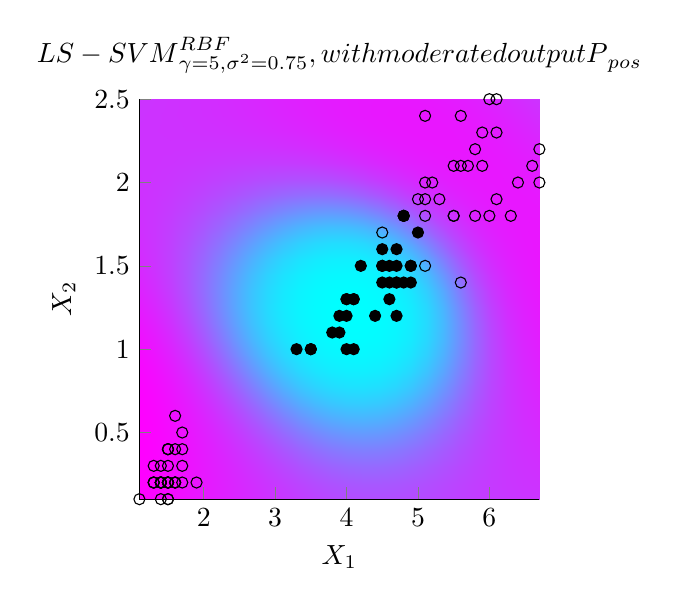
\begin{tikzpicture}

\begin{axis}[%
width=2in,
height=2in,
scale only axis,
xmin=1.1,
xmax=6.7,
xlabel={$\text{X}_\text{1}$},
ymin=0.1,
ymax=2.5,
ylabel={$\text{X}_\text{2}$},
zmin=0,
zmax=1,
zlabel={Y},
view={0}{90},
title={$\text{LS-SVM}_{\gamma\text{=5, }\sigma{}^\text{2}\text{=0.75}}^{\text{RBF}}\text{, with moderated output P}_{\text{pos}}$},
axis x line*=bottom,
axis y line*=left,
axis z line*=left,
legend style={legend cell align=left,align=left,draw=white!15!black}
]

\addplot3[%
surf,
shader=interp,
colormap={mymap}{[1pt] rgb(0pt)=(0,1,1); rgb(63pt)=(1,0,1)},
mesh/rows=26]
table[row sep=crcr,header=false] {%
%
1.1	0.1	0.990504368461164\\
1.1	0.196	0.992760284685133\\
1.1	0.292	0.993725716265635\\
1.1	0.388	0.993685791098687\\
1.1	0.484	0.992641414734618\\
1.1	0.58	0.990314848547624\\
1.1	0.676	0.986150123718386\\
1.1	0.772	0.979357892867502\\
1.1	0.868	0.969076153518419\\
1.1	0.964	0.954679091535128\\
1.1	1.06	0.936165311561707\\
1.1	1.156	0.914444411290007\\
1.1	1.252	0.891307279340938\\
1.1	1.348	0.868995082273217\\
1.1	1.444	0.849538471550146\\
1.1	1.54	0.834206624944392\\
1.1	1.636	0.823312409919004\\
1.1	1.732	0.816370586980401\\
1.1	1.828	0.812434051128297\\
1.1	1.924	0.810425750991907\\
1.1	2.02	0.809368502918053\\
1.1	2.116	0.808498917749368\\
1.1	2.212	0.807295761455228\\
1.1	2.308	0.805461122915757\\
1.1	2.404	0.802882701345237\\
1.1	2.5	0.799592098153668\\
1.324	0.1	0.972967236681189\\
1.324	0.196	0.97684660319093\\
1.324	0.292	0.978628987593197\\
1.324	0.388	0.978500565721881\\
1.324	0.484	0.976412283507765\\
1.324	0.58	0.972057377872013\\
1.324	0.676	0.964893808857214\\
1.324	0.772	0.954237944946606\\
1.324	0.868	0.939470632326005\\
1.324	0.964	0.920372000743563\\
1.324	1.06	0.897512517015319\\
1.324	1.156	0.872493744890567\\
1.324	1.252	0.847780258977674\\
1.324	1.348	0.826056051797851\\
1.324	1.444	0.809395291553264\\
1.324	1.54	0.798699931471295\\
1.324	1.636	0.793645575665675\\
1.324	1.732	0.793037206866494\\
1.324	1.828	0.795308323289289\\
1.324	1.924	0.798939556444679\\
1.324	2.02	0.802701615957642\\
1.324	2.116	0.805735061358228\\
1.324	2.212	0.807527784064296\\
1.324	2.308	0.807850500674361\\
1.324	2.404	0.806688017236708\\
1.324	2.5	0.804180997589845\\
1.548	0.1	0.950111955215424\\
1.548	0.196	0.95434607796666\\
1.548	0.292	0.955972945998913\\
1.548	0.388	0.954954651152518\\
1.548	0.484	0.951070962032123\\
1.548	0.58	0.943885338429259\\
1.548	0.676	0.932777613970449\\
1.548	0.772	0.917083094137\\
1.548	0.868	0.896386362068618\\
1.548	0.964	0.870968283528176\\
1.548	1.06	0.842256045213216\\
1.548	1.156	0.812948041722783\\
1.548	1.252	0.786518483975525\\
1.548	1.348	0.766199366208011\\
1.548	1.444	0.753972754308091\\
1.548	1.54	0.750101440521448\\
1.548	1.636	0.753321515064088\\
1.548	1.732	0.76145704347073\\
1.548	1.828	0.772116517551889\\
1.548	1.924	0.783218116885488\\
1.548	2.02	0.793245255608119\\
1.548	2.116	0.801270437762343\\
1.548	2.212	0.806850852741422\\
1.548	2.308	0.809891628420468\\
1.548	2.404	0.810530533914225\\
1.548	2.5	0.809058318543877\\
1.772	0.1	0.926316665351488\\
1.772	0.196	0.929541565327584\\
1.772	0.292	0.929704684523774\\
1.772	0.388	0.926498829120122\\
1.772	0.484	0.91943508517376\\
1.772	0.58	0.907820042108916\\
1.772	0.676	0.890833680318501\\
1.772	0.772	0.867779009817106\\
1.772	0.868	0.838558240124582\\
1.772	0.964	0.804298645668456\\
1.772	1.06	0.767795743731039\\
1.772	1.156	0.733292548437319\\
1.772	1.252	0.705425533750916\\
1.772	1.348	0.687816301160483\\
1.772	1.444	0.682065619421692\\
1.772	1.54	0.687530376385984\\
1.772	1.636	0.701774248390461\\
1.772	1.732	0.72139793907677\\
1.772	1.828	0.74294405525096\\
1.772	1.924	0.763591724440129\\
1.772	2.02	0.781469755698671\\
1.772	2.116	0.795615511150229\\
1.772	2.212	0.805744408626678\\
1.772	2.308	0.811995896646193\\
1.772	2.404	0.81474407757691\\
1.772	2.5	0.814487516381263\\
1.996	0.1	0.903254056498306\\
1.996	0.196	0.904336346862761\\
1.996	0.292	0.90173405306007\\
1.996	0.388	0.894810773805167\\
1.996	0.484	0.88270538512709\\
1.996	0.58	0.864350931062825\\
1.996	0.676	0.838667418476171\\
1.996	0.772	0.805035310309823\\
1.996	0.868	0.764061157394343\\
1.996	0.964	0.718349960197224\\
1.996	1.06	0.672659765783161\\
1.996	1.156	0.632957028011955\\
1.996	1.252	0.604717004538377\\
1.996	1.348	0.591455779709892\\
1.996	1.444	0.594111499965532\\
1.996	1.54	0.611134050547601\\
1.996	1.636	0.638967448474895\\
1.996	1.732	0.672867295189887\\
1.996	1.828	0.708003742575367\\
1.996	1.924	0.740497789968208\\
1.996	2.02	0.767952736984597\\
1.996	2.116	0.789377513557846\\
1.996	2.212	0.804761326438166\\
1.996	2.308	0.814619918955586\\
1.996	2.404	0.819681852913576\\
1.996	2.5	0.820731750121748\\
2.22	0.1	0.880864186578937\\
2.22	0.196	0.878805814235627\\
2.22	0.292	0.87213372762628\\
2.22	0.388	0.859787232834637\\
2.22	0.484	0.840419301285562\\
2.22	0.58	0.812517388780919\\
2.22	0.676	0.774833966028239\\
2.22	0.772	0.727239129101453\\
2.22	0.868	0.671811719711816\\
2.22	0.964	0.613452963211125\\
2.22	1.06	0.559159524978291\\
2.22	1.156	0.516036966384179\\
2.22	1.252	0.48936720310225\\
2.22	1.348	0.481844993194413\\
2.22	1.444	0.49375023880248\\
2.22	1.54	0.523179954861411\\
2.22	1.636	0.566053489055415\\
2.22	1.732	0.616439466754912\\
2.22	1.828	0.6677606990113\\
2.22	1.924	0.71450007691095\\
2.22	2.02	0.753342126681978\\
2.22	2.116	0.783190118766573\\
2.22	2.212	0.804439223080061\\
2.22	2.308	0.818170957311431\\
2.22	2.404	0.825625108190052\\
2.22	2.5	0.827970818413988\\
2.444	0.1	0.858509815708999\\
2.444	0.196	0.852346389792424\\
2.444	0.292	0.840254917890493\\
2.444	0.388	0.820639448013841\\
2.444	0.484	0.791584750600672\\
2.444	0.58	0.751198956299916\\
2.444	0.676	0.69847494251612\\
2.444	0.772	0.634652157467585\\
2.444	0.868	0.564378999572663\\
2.444	0.964	0.49538269102234\\
2.444	1.06	0.436173758131432\\
2.444	1.156	0.393344034846546\\
2.444	1.252	0.370505314142967\\
2.444	1.348	0.369001673345117\\
2.444	1.444	0.388915648854168\\
2.444	1.54	0.429109278979163\\
2.444	1.636	0.486221524205857\\
2.444	1.732	0.553806748931472\\
2.444	1.828	0.623233135091075\\
2.444	1.924	0.686430200352427\\
2.444	2.02	0.738400782760707\\
2.444	2.116	0.777696682768358\\
2.444	2.212	0.805248199897136\\
2.444	2.308	0.822939628155128\\
2.444	2.404	0.832714304328713\\
2.444	2.5	0.836237498631304\\
2.668	0.1	0.835619692650913\\
2.668	0.196	0.82441885700556\\
2.668	0.292	0.80557250927142\\
2.668	0.388	0.776868665756265\\
2.668	0.484	0.735861043747779\\
2.668	0.58	0.68063347769305\\
2.668	0.676	0.611306098410353\\
2.668	0.772	0.531786166449294\\
2.668	0.868	0.450162141996294\\
2.668	0.964	0.376353988710824\\
2.668	1.06	0.318326095081478\\
2.668	1.156	0.280077584196774\\
2.668	1.252	0.262564177900446\\
2.668	1.348	0.265842366270555\\
2.668	1.444	0.290464382624267\\
2.668	1.54	0.337202387264215\\
2.668	1.636	0.40498896684427\\
2.668	1.732	0.48821913286564\\
2.668	1.828	0.576334353615487\\
2.668	1.924	0.657593823942149\\
2.668	2.02	0.72410399568346\\
2.668	2.116	0.773574088988538\\
2.668	2.212	0.807575294180906\\
2.668	2.308	0.829071002659592\\
2.668	2.404	0.840920923905916\\
2.668	2.5	0.845394634411261\\
2.892	0.1	0.81201619122076\\
2.892	0.196	0.79497886192785\\
2.892	0.292	0.76824519547578\\
2.892	0.388	0.729002402823892\\
2.892	0.484	0.674533680040166\\
2.892	0.58	0.603645998661024\\
2.892	0.676	0.518864689943731\\
2.892	0.772	0.427886995164432\\
2.892	0.868	0.341894215824995\\
2.892	0.964	0.270828852435284\\
2.892	1.06	0.219678764844289\\
2.892	1.156	0.188776596984959\\
2.892	1.252	0.17664017248493\\
2.892	1.348	0.182593807782516\\
2.892	1.444	0.208032324881073\\
2.892	1.54	0.256097416795285\\
2.892	1.636	0.329191964530019\\
2.892	1.732	0.424347219083904\\
2.892	1.828	0.53002659104725\\
2.892	1.924	0.629925113306416\\
2.892	2.02	0.711717649355218\\
2.892	2.116	0.771549300512273\\
2.892	2.212	0.811717307340864\\
2.892	2.308	0.83656034909138\\
2.892	2.404	0.850055062877292\\
2.892	2.5	0.855152748988043\\
3.116	0.1	0.788066645618553\\
3.116	0.196	0.764701248288884\\
3.116	0.292	0.729431783594707\\
3.116	0.388	0.679008816806025\\
3.116	0.484	0.610959325588232\\
3.116	0.58	0.525823396596255\\
3.116	0.676	0.429657291939644\\
3.116	0.772	0.333974962805274\\
3.116	0.868	0.251135676020566\\
3.116	0.964	0.188523084958025\\
3.116	1.06	0.146996372547768\\
3.116	1.156	0.123767749268064\\
3.116	1.252	0.11595459486621\\
3.116	1.348	0.12272409997665\\
3.116	1.444	0.146226836922153\\
3.116	1.54	0.191601861045657\\
3.116	1.636	0.264942925107424\\
3.116	1.732	0.367411347384958\\
3.116	1.828	0.488124804197609\\
3.116	1.924	0.605986592721132\\
3.116	2.02	0.702789106137177\\
3.116	2.116	0.772365767655613\\
3.116	2.212	0.817857897405732\\
3.116	2.308	0.845258863038618\\
3.116	2.404	0.859796653558342\\
3.116	2.5	0.865115914425039\\
3.34	0.1	0.76468790501271\\
3.34	0.196	0.734999740726407\\
3.34	0.292	0.691303038974505\\
3.34	0.388	0.630210993168803\\
3.34	0.484	0.550123641390086\\
3.34	0.58	0.45416246240064\\
3.34	0.676	0.352190215441672\\
3.34	0.772	0.25820945755033\\
3.34	0.868	0.183365923086473\\
3.34	0.964	0.13114866631097\\
3.34	1.06	0.0988549503389776\\
3.34	1.156	0.0819309789621784\\
3.34	1.252	0.0770899584988685\\
3.34	1.348	0.0836578727093823\\
3.34	1.444	0.104249418981132\\
3.34	1.54	0.145278035297611\\
3.34	1.636	0.21592783655427\\
3.34	1.732	0.322013829064894\\
3.34	1.828	0.454789293886062\\
3.34	1.924	0.588765021104021\\
3.34	2.02	0.699006390907767\\
3.34	2.116	0.776680758998878\\
3.34	2.212	0.826025243147024\\
3.34	2.308	0.854885853145758\\
3.34	2.404	0.869740557831728\\
3.34	2.5	0.874840596615701\\
3.564	0.1	0.743203711118345\\
3.564	0.196	0.707824078991763\\
3.564	0.292	0.656706362194081\\
3.564	0.388	0.586654586172646\\
3.564	0.484	0.497403785618912\\
3.564	0.58	0.394888294395728\\
3.564	0.676	0.292024384322457\\
3.564	0.772	0.203471483856332\\
3.564	0.868	0.137755251727483\\
3.564	0.964	0.0947780290762102\\
3.564	1.06	0.069625898797338\\
3.564	1.156	0.057133107518748\\
3.564	1.252	0.0541562770927531\\
3.564	1.348	0.0602741341324957\\
3.564	1.444	0.0783482223676206\\
3.564	1.54	0.115511465787889\\
3.564	1.636	0.183213005627436\\
3.564	1.732	0.291438890581377\\
3.564	1.828	0.433953776258181\\
3.564	1.924	0.581275973728251\\
3.564	2.02	0.70190909682757\\
3.564	2.116	0.784901202163077\\
3.564	2.212	0.836043793595789\\
3.564	2.308	0.865050192090465\\
3.564	2.404	0.879446660729306\\
3.564	2.5	0.883891970988788\\
3.788	0.1	0.725083259925919\\
3.788	0.196	0.685279708402496\\
3.788	0.292	0.628583435295115\\
3.788	0.388	0.552198990621985\\
3.788	0.484	0.457244365240955\\
3.788	0.58	0.351956446777856\\
3.788	0.676	0.251025741994199\\
3.788	0.772	0.168512540140335\\
3.788	0.868	0.110333987637109\\
3.788	0.964	0.0739819639245475\\
3.788	1.06	0.0535240178037277\\
3.788	1.156	0.0437932361148091\\
3.788	1.252	0.0419567029985279\\
3.788	1.348	0.0478497034885524\\
3.788	1.444	0.0645391378275711\\
3.788	1.54	0.0996966926961787\\
3.788	1.636	0.166457172074332\\
3.788	1.732	0.277859285828153\\
3.788	1.828	0.428956620010464\\
3.788	1.924	0.586031853642575\\
3.788	2.02	0.712480135633581\\
3.788	2.116	0.796998884108846\\
3.788	2.212	0.847504103078603\\
3.788	2.308	0.875283174519133\\
3.788	2.404	0.888485273110229\\
3.788	2.5	0.891884596685172\\
4.012	0.1	0.711633932348413\\
4.012	0.196	0.669193345259075\\
4.012	0.292	0.609371544767288\\
4.012	0.388	0.529776549423247\\
4.012	0.484	0.432500241882705\\
4.012	0.58	0.327064763628113\\
4.012	0.676	0.228740992328414\\
4.012	0.772	0.150687413053473\\
4.012	0.868	0.0971600877642768\\
4.012	0.964	0.0645152286502779\\
4.012	1.06	0.0465501969287329\\
4.012	1.156	0.0382958020941647\\
4.012	1.252	0.0372094383621259\\
4.012	1.348	0.0433903895192557\\
4.012	1.444	0.0602377904003332\\
4.012	1.54	0.0961236715739318\\
4.012	1.636	0.165611899665547\\
4.012	1.732	0.283198564745813\\
4.012	1.828	0.442370270497163\\
4.012	1.924	0.604419550110707\\
4.012	2.02	0.730717505118266\\
4.012	2.116	0.812381769126644\\
4.012	2.212	0.859777199143516\\
4.012	2.308	0.885081581103184\\
4.012	2.404	0.896469881253643\\
4.012	2.5	0.898500765806527\\
4.236	0.1	0.703737397932287\\
4.236	0.196	0.660761860564883\\
4.236	0.292	0.600592768524454\\
4.236	0.388	0.521071172958358\\
4.236	0.484	0.424561235444923\\
4.236	0.58	0.320669775839079\\
4.236	0.676	0.224346862389428\\
4.236	0.772	0.148185404938231\\
4.236	0.868	0.0960665622433177\\
4.236	0.964	0.0643308121405882\\
4.236	1.06	0.0469593757079941\\
4.236	1.156	0.0392034165696254\\
4.236	1.252	0.0387517576277931\\
4.236	1.348	0.0460329071380193\\
4.236	1.444	0.0650507600868837\\
4.236	1.54	0.10525092705465\\
4.236	1.636	0.182374126636493\\
4.236	1.732	0.309901508816835\\
4.236	1.828	0.475637343099097\\
4.236	1.924	0.636032642414745\\
4.236	2.02	0.755360851061026\\
4.236	2.116	0.829907699230279\\
4.236	2.212	0.872087152500713\\
4.236	2.308	0.893955059060348\\
4.236	2.404	0.903073352693481\\
4.236	2.5	0.903487543248426\\
4.46	0.1	0.701691689288449\\
4.46	0.196	0.660359583304887\\
4.46	0.292	0.602678522987204\\
4.46	0.388	0.526511108865222\\
4.46	0.484	0.433765087854006\\
4.46	0.58	0.332977852478857\\
4.46	0.676	0.237991580870683\\
4.46	0.772	0.161227599739734\\
4.46	0.868	0.107424808519471\\
4.46	0.964	0.0739596167195332\\
4.46	1.06	0.0554406209145291\\
4.46	1.156	0.0474008441576959\\
4.46	1.252	0.0477716929050729\\
4.46	1.348	0.0574775784169518\\
4.46	1.444	0.081511998700021\\
4.46	1.54	0.130707981389993\\
4.46	1.636	0.220954815171913\\
4.46	1.732	0.360643898035418\\
4.46	1.828	0.528047159975066\\
4.46	1.924	0.678162026389944\\
4.46	2.02	0.783974974730555\\
4.46	2.116	0.848078887894852\\
4.46	2.212	0.883627293766937\\
4.46	2.308	0.901466976604155\\
4.46	2.404	0.908027423060121\\
4.46	2.5	0.906638567851189\\
4.684	0.1	0.705177036572286\\
4.684	0.196	0.667504501154754\\
4.684	0.292	0.614955716911305\\
4.684	0.388	0.545312520138768\\
4.684	0.484	0.45953828431175\\
4.684	0.58	0.36418769623682\\
4.684	0.676	0.271107366443453\\
4.684	0.772	0.192438127710471\\
4.684	0.868	0.134596689010165\\
4.684	0.964	0.0970619210651548\\
4.684	1.06	0.0757765747847597\\
4.684	1.156	0.0668794533923531\\
4.684	1.252	0.0687490529164698\\
4.684	1.348	0.0831000161796847\\
4.684	1.444	0.11623607814502\\
4.684	1.54	0.179938086184153\\
4.684	1.636	0.287208469458816\\
4.684	1.732	0.436039932927331\\
4.684	1.828	0.595270556071396\\
4.684	1.924	0.7259290915266\\
4.684	2.02	0.813480870013296\\
4.684	2.116	0.865359568420269\\
4.684	2.212	0.893678705457754\\
4.684	2.308	0.907256759532961\\
4.684	2.404	0.911107939143804\\
4.684	2.5	0.907768343858442\\
4.908	0.1	0.713331053430887\\
4.908	0.196	0.680954391461074\\
4.908	0.292	0.635731852521139\\
4.908	0.388	0.575448982454721\\
4.908	0.484	0.500061038308246\\
4.908	0.58	0.413727131266725\\
4.908	0.676	0.325433436104958\\
4.908	0.772	0.24616449534314\\
4.908	0.868	0.183927790204292\\
4.908	0.964	0.141116477390391\\
4.908	1.06	0.116058250567997\\
4.908	1.156	0.106296664753246\\
4.908	1.252	0.111185011727726\\
4.908	1.348	0.133528861799285\\
4.908	1.444	0.180557404744444\\
4.908	1.54	0.262519219410285\\
4.908	1.636	0.384208434608729\\
4.908	1.732	0.530730319079807\\
4.908	1.828	0.668966850200209\\
4.908	1.924	0.773462052822969\\
4.908	2.02	0.840956879284778\\
4.908	2.116	0.880480305706532\\
4.908	2.212	0.901685808033091\\
4.908	2.308	0.911037240323869\\
4.908	2.404	0.912110741952351\\
4.908	2.5	0.906686802448387\\
5.132	0.1	0.724905519861028\\
5.132	0.196	0.6989109717992\\
5.132	0.292	0.662498511327816\\
5.132	0.388	0.613680961304662\\
5.132	0.484	0.55175649430751\\
5.132	0.58	0.478776171808317\\
5.132	0.676	0.400551802521887\\
5.132	0.772	0.325717495308677\\
5.132	0.868	0.262627552021425\\
5.132	0.964	0.216418060488429\\
5.132	1.06	0.188683326365731\\
5.132	1.156	0.179493797304686\\
5.132	1.252	0.189880099678477\\
5.132	1.348	0.223471405696553\\
5.132	1.444	0.28622939689437\\
5.132	1.54	0.382172107367991\\
5.132	1.636	0.504555210304922\\
5.132	1.732	0.631686317247812\\
5.132	1.828	0.739102291300538\\
5.132	1.924	0.815714528154674\\
5.132	2.02	0.864311464108727\\
5.132	2.116	0.892601306021845\\
5.132	2.212	0.907267109438967\\
5.132	2.308	0.91257026246845\\
5.132	2.404	0.91082554950208\\
5.132	2.5	0.90318213138049\\
5.356	0.1	0.738470133078472\\
5.356	0.196	0.71930862087525\\
5.356	0.292	0.692299502716522\\
5.356	0.388	0.655902819504551\\
5.356	0.484	0.609283254673067\\
5.356	0.58	0.553209226457914\\
5.356	0.676	0.490927369206433\\
5.356	0.772	0.428241314951064\\
5.356	0.868	0.372230392670077\\
5.356	0.964	0.329240380958435\\
5.356	1.06	0.303694826502835\\
5.356	1.156	0.298505544055743\\
5.356	1.252	0.316309375421961\\
5.356	1.348	0.359980083712454\\
5.356	1.444	0.43089264629513\\
5.356	1.54	0.524647711816809\\
5.356	1.636	0.627984310897152\\
5.356	1.732	0.723192174599875\\
5.356	1.828	0.797950188218138\\
5.356	1.924	0.84978219501872\\
5.356	2.02	0.882513100922709\\
5.356	2.116	0.90129867507549\\
5.356	2.212	0.91017156968181\\
5.356	2.308	0.911632347724885\\
5.356	2.404	0.907017520620816\\
5.356	2.5	0.897020887937715\\
5.58	0.1	0.752621027836463\\
5.58	0.196	0.740135263419828\\
5.58	0.292	0.72222633605273\\
5.58	0.388	0.69788695238876\\
5.58	0.484	0.666527525552648\\
5.58	0.58	0.628468252281596\\
5.58	0.676	0.585497992735905\\
5.58	0.772	0.54119096630855\\
5.58	0.868	0.500617600474229\\
5.58	0.964	0.469425255755284\\
5.58	1.06	0.452788967102778\\
5.58	1.156	0.454772165947783\\
5.58	1.252	0.477994063621309\\
5.58	1.348	0.522890059770635\\
5.58	1.444	0.586193222913574\\
5.58	1.54	0.65984076045526\\
5.58	1.636	0.732683967223362\\
5.58	1.732	0.795066704372174\\
5.58	1.828	0.84241201731224\\
5.58	1.924	0.874984132739906\\
5.58	2.02	0.895386930870221\\
5.58	2.116	0.906432156575631\\
5.58	2.212	0.910211497935162\\
5.58	2.308	0.907986676600487\\
5.58	2.404	0.900428257982989\\
5.58	2.5	0.88797550450931\\
5.804	0.1	0.766150458920649\\
5.804	0.196	0.759705137586122\\
5.804	0.292	0.749887518409751\\
5.804	0.388	0.736146748332531\\
5.804	0.484	0.718227025311629\\
5.804	0.58	0.696424517727001\\
5.804	0.676	0.671884234813322\\
5.804	0.772	0.646821304319164\\
5.804	0.868	0.624495557180897\\
5.804	0.964	0.608821303992224\\
5.804	1.06	0.603658305505224\\
5.804	1.156	0.611953210382895\\
5.804	1.252	0.634867776205604\\
5.804	1.348	0.671015153502223\\
5.804	1.444	0.71618232751566\\
5.804	1.54	0.76415702870021\\
5.804	1.636	0.808711564409488\\
5.804	1.732	0.845601717943979\\
5.804	1.828	0.873250706747875\\
5.804	1.924	0.892051016747809\\
5.804	2.02	0.903222788856824\\
5.804	2.116	0.907985710257829\\
5.804	2.212	0.907205556376914\\
5.804	2.308	0.901378709815298\\
5.804	2.404	0.890809207110329\\
5.804	2.5	0.875887938758477\\
6.028	0.1	0.778147506335644\\
6.028	0.196	0.776814758438399\\
6.028	0.292	0.773680962990459\\
6.028	0.388	0.768483787743559\\
6.028	0.484	0.76118074780454\\
6.028	0.58	0.752077487718036\\
6.028	0.676	0.741958599284304\\
6.028	0.772	0.732171406564383\\
6.028	0.868	0.724586741777415\\
6.028	0.964	0.721364863974563\\
6.028	1.06	0.724509396487916\\
6.028	1.156	0.735285900492166\\
6.028	1.252	0.753681012721799\\
6.028	1.348	0.778149358501218\\
6.028	1.444	0.805872706174325\\
6.028	1.54	0.833537976708916\\
6.028	1.636	0.858284875998182\\
6.028	1.732	0.878317719772763\\
6.028	1.828	0.892942535061971\\
6.028	1.924	0.902201044707922\\
6.028	2.02	0.906428733828575\\
6.028	2.116	0.905949293680375\\
6.028	2.212	0.900958278536269\\
6.028	2.308	0.891571721927025\\
6.028	2.404	0.877997900997378\\
6.028	2.5	0.860770045171803\\
6.252	0.1	0.788024741260862\\
6.252	0.196	0.790764732607962\\
6.252	0.292	0.792809154040381\\
6.252	0.388	0.794015700546898\\
6.252	0.484	0.794388178667878\\
6.252	0.58	0.79413541046816\\
6.252	0.676	0.793713399245031\\
6.252	0.772	0.793828270200054\\
6.252	0.868	0.795371818634255\\
6.252	0.964	0.799268548827218\\
6.252	1.06	0.806242115938539\\
6.252	1.156	0.816557598627374\\
6.252	1.252	0.829841234164803\\
6.252	1.348	0.84508216336726\\
6.252	1.444	0.860851888985917\\
6.252	1.54	0.875658622726648\\
6.252	1.636	0.888270719335739\\
6.252	1.732	0.897872348325178\\
6.252	1.828	0.904030265375527\\
6.252	1.924	0.906551087280082\\
6.252	2.02	0.90533172531218\\
6.252	2.116	0.900273790619467\\
6.252	2.212	0.891293892167666\\
6.252	2.308	0.878433046682992\\
6.252	2.404	0.862035919238922\\
6.252	2.5	0.842922652630744\\
6.476	0.1	0.795488873213357\\
6.476	0.196	0.801283511186994\\
6.476	0.292	0.807110043108044\\
6.476	0.388	0.812830436116497\\
6.476	0.484	0.818381142337909\\
6.476	0.58	0.823800940680073\\
6.476	0.676	0.82924024128245\\
6.476	0.772	0.834943357233725\\
6.476	0.868	0.841198436875431\\
6.476	0.964	0.848257438128123\\
6.476	1.06	0.856241401689989\\
6.476	1.156	0.865060180855467\\
6.476	1.252	0.874380806024825\\
6.476	1.348	0.883664999865412\\
6.476	1.444	0.89226542235116\\
6.476	1.54	0.899539857801974\\
6.476	1.636	0.904935160175997\\
6.476	1.732	0.908014144231914\\
6.476	1.828	0.908432079200715\\
6.476	1.924	0.905893457594775\\
6.476	2.02	0.900126484082259\\
6.476	2.116	0.890907239213525\\
6.476	2.212	0.878151578358104\\
6.476	2.308	0.86206577089766\\
6.476	2.404	0.843302928211407\\
6.476	2.5	0.823030008529183\\
6.7	0.1	0.80048334159291\\
6.7	0.196	0.808411254041814\\
6.7	0.292	0.816829404978146\\
6.7	0.388	0.82554947614677\\
6.7	0.484	0.834397839831099\\
6.7	0.58	0.843236758267029\\
6.7	0.676	0.851973531068651\\
6.7	0.772	0.860554104731485\\
6.7	0.868	0.868942001355271\\
6.7	0.964	0.877088107525869\\
6.7	1.06	0.884900547340904\\
6.7	1.156	0.892224812482909\\
6.7	1.252	0.898841067108871\\
6.7	1.348	0.904478423714215\\
6.7	1.444	0.908838178927339\\
6.7	1.54	0.911614171786466\\
6.7	1.636	0.912501348259957\\
6.7	1.732	0.911191973457901\\
6.7	1.828	0.907368758425509\\
6.7	1.924	0.900711945841691\\
6.7	2.02	0.8909408483841\\
6.7	2.116	0.877905912658527\\
6.7	2.212	0.861728656596225\\
6.7	2.308	0.842950392616072\\
6.7	2.404	0.822610676835024\\
6.7	2.5	0.802170896787991\\
};
\addplot3 [color=black,only marks,mark=o]
 table[row sep=crcr] {%
1.5	0.3	1\\
1.5	0.2	1\\
6	2.5	1\\
6.7	2	1\\
4.8	1.8	1\\
1.5	0.2	1\\
1.9	0.2	1\\
1.3	0.3	1\\
1.5	0.2	1\\
5	1.9	1\\
1.4	0.3	1\\
5.8	2.2	1\\
5.1	2.4	1\\
4.8	1.8	1\\
6.6	2.1	1\\
5.1	1.9	1\\
5.6	1.4	1\\
1.7	0.5	1\\
1.5	0.2	1\\
1.3	0.2	1\\
1.6	0.2	1\\
1.4	0.2	1\\
5.6	2.4	1\\
1.6	0.6	1\\
1.3	0.2	1\\
5.5	1.8	1\\
6.1	2.5	1\\
1.5	0.4	1\\
5.1	1.8	1\\
5.9	2.1	1\\
6	1.8	1\\
1.5	0.1	1\\
5.9	2.3	1\\
5.6	2.1	1\\
5.1	2	1\\
1.5	0.4	1\\
6.1	2.3	1\\
1.6	0.2	1\\
5.2	2	1\\
1.5	0.1	1\\
6.4	2	1\\
1.4	0.2	1\\
1.4	0.2	1\\
5.5	1.8	1\\
1.4	0.2	1\\
1.7	0.2	1\\
1.5	0.2	1\\
4.5	1.7	1\\
1.4	0.1	1\\
6.1	1.9	1\\
5.5	2.1	1\\
1.3	0.2	1\\
1.5	0.4	1\\
1.7	0.4	1\\
5.8	1.8	1\\
1.6	0.2	1\\
5.1	1.5	1\\
1.1	0.1	1\\
1.4	0.2	1\\
1.7	0.3	1\\
1.6	0.4	1\\
5.7	2.1	1\\
6.7	2.2	1\\
6.3	1.8	1\\
5.3	1.9	1\\
1.5	0.2	1\\
1.4	0.2	1\\
};

\addplot3 [color=black,only marks,mark=*,mark options={solid}]
 table[row sep=crcr] {%
5	1.7	1\\
4.5	1.5	1\\
3.9	1.2	1\\
3.3	1	1\\
4.5	1.4	1\\
4.8	1.8	1\\
4	1.3	1\\
3.5	1	1\\
4.9	1.4	1\\
4.1	1.3	1\\
4.5	1.5	1\\
4.6	1.4	1\\
4.7	1.4	1\\
4.7	1.6	1\\
4.8	1.4	1\\
3.5	1	1\\
3.9	1.1	1\\
3.8	1.1	1\\
4.7	1.2	1\\
4.6	1.5	1\\
4	1	1\\
4	1.3	1\\
4.4	1.2	1\\
4.5	1.6	1\\
4.1	1	1\\
4.7	1.4	1\\
4	1.2	1\\
4.9	1.5	1\\
4.7	1.5	1\\
4.1	1.3	1\\
4.9	1.5	1\\
4.2	1.5	1\\
4.6	1.3	1\\
};


\end{axis}
\end{tikzpicture}%
\end{document}

\caption{Posterior class probabilities of an iris data classification svm}
\label{fig:bayesianClass}
\end{figure}
Bayesian inference can also be used for input relevance detection. This is done using radial basis function kernels with a different width for each kernel on the third level of inference. Inputs which end up with small kernel width are successively removed as small density is a strong indication for data memorization. 
\begin{figure}
\centering
% This file was created by matlab2tikz.
% Minimal pgfplots version: 1.3
%
%The latest updates can be retrieved from
%  http://www.mathworks.com/matlabcentral/fileexchange/22022-matlab2tikz
%where you can also make suggestions and rate matlab2tikz.
%
\documentclass[tikz]{standalone}
\usepackage{pgfplots}
\usepackage{grffile}
\pgfplotsset{compat=newest}
\usetikzlibrary{plotmarks}
\usepackage{amsmath}

\begin{document}
\definecolor{mycolor1}{rgb}{0.00000,0.44700,0.74100}%
\definecolor{mycolor2}{rgb}{0.85000,0.32500,0.09800}%
%
\begin{tikzpicture}

\begin{axis}[%
width=1.5in,
height=1.5in,
scale only axis,
xmin=-4,
xmax=8,
ymin=-2,
ymax=3
]
\addplot [color=mycolor1,only marks,mark=*,mark options={solid},forget plot]
  table[row sep=crcr]{%
2.23173950113028	-0.707235664131701\\
-1.75283441669061	-1.26352273508506\\
1.52696285403787	-1.25701242564515\\
6.92595860667378	1.14703110506583\\
0.992288259401783	0.355691348773115\\
-2.38088283243344	-0.377059650914444\\
-0.0703874402718037	2.73138364182116\\
2.52271825080349	-0.15441451909862\\
4.40127279264061	-0.974245608889248\\
0.184044968367855	2.08705218977923\\
1.93858175306489	-0.855316544704607\\
3.28668641699644	0.15127163588402\\
4.53146300574143	-1.19720396951798\\
3.93887330240748	-1.24560144788979\\
-1.63119465735655	-1.0474678018861\\
6.06962104678691	1.44243647785188\\
0.788765882876157	0.643253176717919\\
2.29622209285288	-0.935893512595936\\
6.88615001590479	1.12876831062751\\
6.5820931345633	2.26117952838564\\
5.1764607651304	0.206898830437358\\
1.23895470686491	0.129358752491145\\
5.17976533449552	-0.267957430514004\\
1.44495886655101	-1.38184986876009\\
0.80260347416991	1.04943474419511\\
4.07235169146731	-0.740472590455723\\
-0.610838808048535	1.21568481283561\\
-1.24234887361512	-0.851905923649427\\
-0.618532324826298	1.16574397574468\\
-0.164083812809716	1.67012386104317\\
-2.59351286265993	-0.453921952626963\\
2.51416683951155	-0.723564974885692\\
6.42498982581975	1.79065899076159\\
4.87836608192952	-0.289120821051555\\
-0.585677776717266	1.81772626450483\\
3.95975547553569	-0.909952936075635\\
-2.84742490747308	-0.283220831620656\\
4.68547506744655	-0.816023261073292\\
0.318926908734118	1.99359678024607\\
0.223300939983337	1.40308953928427\\
4.65437295434549	-1.28520895197063\\
0.841649712749959	0.210924513526393\\
-0.813732790099592	0.769044200347363\\
2.63322082264663	0.0382833070552852\\
-0.793666747480569	0.571957099127607\\
-1.37362945527807	-0.545017671953214\\
0.996400500930371	-0.0887416779171835\\
-2.7960505893699	-0.304957906566694\\
1.23270130284549	-0.0648006801425405\\
-2.96726700088416	0.0148218595150724\\
-2.55139971305841	-0.283295589293754\\
-1.10875884853879	0.107327998446395\\
-0.986636680030804	-0.159357712734728\\
3.00349620129511	0.224424601274896\\
-0.682775420740311	0.752704141382259\\
2.66547879788075	-0.0144810835422538\\
2.50749671427242	-0.23973098540769\\
0.380062938437166	2.05775158636282\\
6.89923506936783	1.27989220636882\\
-1.51640749638593	-0.709406768032139\\
5.51287667320353	0.617852553425281\\
4.87180010527188	-1.23372023239646\\
2.24300977638559	-1.00016740102341\\
-2.81161037756785	0.0507909731278836\\
-0.365482848054219	1.54118422896584\\
6.98589723414933	0.964693761359243\\
4.10540617746818	-0.597545326223692\\
-0.819096652105084	1.08742183923307\\
3.41612687350768	-0.132674902075258\\
-1.7893175161328	-1.3723699379554\\
2.56681340271155	-0.643156110303212\\
4.87968206543568	-0.212837543619907\\
1.14501925417731	-0.80021235648644\\
-2.16335593938898	-0.872248734113941\\
2.87106720646176	-0.203469391213842\\
3.39266464024492	-0.119003070576024\\
-1.74845268652181	-1.64757171327009\\
5.65261678105272	0.672565081349719\\
1.8778428565265	-0.64447864092002\\
-0.239821813217713	1.33211560055689\\
0.114716359508689	2.42202055521875\\
3.66566706759921	-0.460542994994516\\
2.00098078791296	-1.14206054097244\\
1.44138521478666	-0.947979920777616\\
0.255825094713326	1.56245338843893\\
2.65923689643975	-0.105698194733239\\
-2.8477728491269	-0.227017537561069\\
2.52833547476891	-0.365638627277357\\
6.35824215383956	2.27419223939399\\
1.81772301596827	-1.02272011111503\\
0.284756515265967	1.79253956440656\\
5.03081686629851	-0.100721806375066\\
-1.56534434798748	-1.34752828192995\\
-2.2137724839069	-1.17350445054142\\
1.45407925813256	-0.91152299253964\\
1.65510336176384	-1.62396990908303\\
4.36678637754769	-0.93143115653883\\
3.99037204178715	-0.962092427145375\\
2.33090326961467	-0.8419018258242\\
-0.936768196500439	0.122434774369135\\
};
\addplot [color=mycolor2,solid,forget plot]
  table[row sep=crcr]{%
-2.96726700088416	-0.0450094015721925\\
-2.86726700088416	-0.109379403806043\\
-2.76726700088416	-0.198146879571399\\
-2.66726700088416	-0.306821315156906\\
-2.56726700088416	-0.429840736320218\\
-2.46726700088416	-0.560805731081447\\
-2.36726700088416	-0.692749511788654\\
-2.26726700088416	-0.818433100680475\\
-2.16726700088416	-0.930653696557052\\
-2.06726700088416	-1.02255373140321\\
-1.96726700088416	-1.0879180769974\\
-1.86726700088416	-1.12144731484499\\
-1.76726700088416	-1.1189959203147\\
-1.66726700088416	-1.07776559642192\\
-1.56726700088416	-0.996445769236892\\
-1.46726700088416	-0.875295354688978\\
-1.36726700088416	-0.71616224204473\\
-1.26726700088416	-0.522439419507015\\
-1.16726700088416	-0.298959193366112\\
-1.06726700088416	-0.0518294232282358\\
-0.967267000884161	0.211781986493534\\
-0.867267000884161	0.483906026874361\\
-0.767267000884161	0.756064901417241\\
-0.667267000884161	1.01958631949472\\
-0.567267000884161	1.26592747310318\\
-0.467267000884161	1.48699599841861\\
-0.367267000884161	1.67545532239863\\
-0.267267000884161	1.82500239378536\\
-0.167267000884161	1.93060687367781\\
-0.0672670008841609	1.98870237072156\\
0.0327329991158387	1.99732218998028\\
0.132732999115839	1.95617424787512\\
0.232732999115839	1.86665220145068\\
0.332732999115839	1.73178235342636\\
0.432732999115839	1.55610842512402\\
0.532732999115839	1.34551873683619\\
0.632732999115839	1.10702260223572\\
0.732732999115839	0.84848473993711\\
0.832732999115839	0.578328151990286\\
0.932732999115839	0.305217150540272\\
1.03273299911584	0.0377329812846829\\
1.13273299911584	-0.215945234648927\\
1.23273299911584	-0.448341750863983\\
1.33273299911584	-0.652955876049908\\
1.43273299911584	-0.824493516813866\\
1.53273299911584	-0.959049628069304\\
1.63273299911584	-1.05423458310584\\
1.73273299911584	-1.10923971823791\\
1.83273299911584	-1.12483973594861\\
1.93273299911584	-1.10333216883156\\
2.03273299911584	-1.04841661397673\\
2.13273299911584	-0.965018843803327\\
2.23273299911584	-0.859067089228436\\
2.33273299911584	-0.737229687246011\\
2.43273299911584	-0.606624811988159\\
2.53273299911584	-0.474514105405821\\
2.63273299911584	-0.347992647260337\\
2.73273299911584	-0.233687829485573\\
2.83273299911584	-0.137479322369303\\
2.93273299911584	-0.0642514546928986\\
3.03273299911584	-0.017688011701221\\
3.13273299911584	-0.000117736365372934\\
3.23273299911584	-0.0124167696302319\\
3.33273299911584	-0.0539719662080897\\
3.43273299911584	-0.122706565939642\\
3.53273299911584	-0.215167185024465\\
3.63273299911584	-0.326668617116538\\
3.73273299911584	-0.451490600325627\\
3.83273299911584	-0.58311860590219\\
3.93273299911584	-0.714518921827964\\
4.03273299911584	-0.838436911026728\\
4.13273299911584	-0.947706375267176\\
4.23273299911584	-1.03555749011898\\
4.33273299911584	-1.09591081233994\\
4.43273299911584	-1.12364539758981\\
4.53273299911584	-1.1148300821833\\
4.63273299911584	-1.06690843737588\\
4.73273299911584	-0.978829740561869\\
4.83273299911584	-0.851120451674077\\
4.93273299911584	-0.685893049618872\\
5.03273299911584	-0.486791578467003\\
5.13273299911584	-0.258875776909141\\
5.23273299911584	-0.00844811655410244\\
5.33273299911584	0.257169642794621\\
5.43273299911584	0.529901750765557\\
5.53273299911584	0.80121530612681\\
5.63273299911584	1.06243705545253\\
5.73273299911584	1.30507775460223\\
5.83273299911584	1.52115137570359\\
5.93273299911584	1.70347662602738\\
6.03273299911584	1.84594892659656\\
6.13273299911584	1.94377215065006\\
6.23273299911584	1.99364099950157\\
6.33273299911584	1.99386683327547\\
6.43273299911584	1.94444199940712\\
6.53273299911584	1.84704012423049\\
6.63273299911584	1.70495235616353\\
6.73273299911584	1.52296207264504\\
6.83273299911584	1.30716298676483\\
6.93273299911584	1.06472781712749\\
};
\end{axis}
\end{tikzpicture}%
\end{document}
% This file was created by matlab2tikz.
% Minimal pgfplots version: 1.3
%
%The latest updates can be retrieved from
%  http://www.mathworks.com/matlabcentral/fileexchange/22022-matlab2tikz
%where you can also make suggestions and rate matlab2tikz.
%
\documentclass[tikz]{standalone}
\usepackage{pgfplots}
\usepackage{grffile}
\pgfplotsset{compat=newest}
\usetikzlibrary{plotmarks}
\usepackage{amsmath}

\begin{document}
\definecolor{mycolor1}{rgb}{0.00000,0.44700,0.74100}%
\definecolor{mycolor2}{rgb}{0.85000,0.32500,0.09800}%
%
\begin{tikzpicture}

\begin{axis}[%
width=1.5in,
height=1.5in,
scale only axis,
xmin=-4,
xmax=8,
ymin=-2,
ymax=3
]
\addplot [color=mycolor1,only marks,mark=*,mark options={solid},forget plot]
  table[row sep=crcr]{%
-1.43032754740803	-0.707235664131701\\
1.02239519762668	-1.26352273508506\\
1.37575868338577	-1.25701242564515\\
6.75063468894014	1.14703110506583\\
6.26744192452944	0.355691348773115\\
0.0806415174070532	-0.377059650914444\\
5.62582601622939	2.73138364182116\\
2.60227281225362	-0.15441451909862\\
2.441622817794	-0.974245608889248\\
5.42279598560883	2.08705218977923\\
4.87970869649794	-0.855316544704607\\
2.36371208102865	0.15127163588402\\
-2.98169616127871	-1.19720396951798\\
0.701524666339668	-1.24560144788979\\
1.36120802744759	-1.0474678018861\\
3.3320250489121	1.44243647785188\\
-1.5322260345508	0.643253176717919\\
2.65367033193397	-0.935893512595936\\
1.03116857984051	1.12876831062751\\
-2.46018191482205	2.26117952838564\\
-1.64015280225135	0.206898830437358\\
0.90509652996561	0.129358752491145\\
1.57555564498429	-0.267957430514004\\
0.31911062224268	-1.38184986876009\\
5.57332663054989	1.04943474419511\\
3.07155815474691	-0.740472590455723\\
-1.0288166719467	1.21568481283561\\
-1.56478909438691	-0.851905923649427\\
4.67379950824231	1.16574397574468\\
3.52723109508908	1.67012386104317\\
0.422798805365599	-0.453921952626963\\
-2.43388959300972	-0.723564974885692\\
1.20361597358419	1.79065899076159\\
1.60863802875603	-0.289120821051555\\
2.35502643550151	1.81772626450483\\
5.28422805979749	-0.909952936075635\\
6.9837009190541	-0.283220831620656\\
0.824054587947423	-0.816023261073292\\
-1.09920018228761	1.99359678024607\\
6.92391333780454	1.40308953928427\\
3.79936803126806	-1.28520895197063\\
6.34896023577981	0.210924513526393\\
3.36410175625084	0.769044200347363\\
3.48704621905513	0.0382833070552852\\
0.82611717672659	0.571957099127607\\
-2.72126393954721	-0.545017671953214\\
2.93066375584962	-0.0887416779171835\\
4.31305229694702	-0.304957906566694\\
3.53124293686903	-0.0648006801425405\\
-2.38038404351335	0.0148218595150724\\
-1.46959210460174	-0.283295589293754\\
4.55653792294532	0.107327998446395\\
1.95833218424375	-0.159357712734728\\
0.843690791639575	0.224424601274896\\
-0.116821777825012	0.752704141382259\\
-1.13633535570925	-0.0144810835422538\\
6.47337577515949	-0.23973098540769\\
0.980563902621672	2.05775158636282\\
-1.60848318875553	1.27989220636882\\
2.41372661862117	-0.709406768032139\\
-2.69483604914573	0.617852553425281\\
2.48450043884377	-1.23372023239646\\
0.96588617462299	-1.00016740102341\\
4.60945615012275	0.0507909731278836\\
-1.3721541797454	1.54118422896584\\
1.68100120595734	0.964693761359243\\
2.93644658893117	-0.597545326223692\\
-2.14665623210863	1.08742183923307\\
1.97140759324717	-0.132674902075258\\
4.76898758063257	-1.3723699379554\\
-1.66182077557351	-0.643156110303212\\
4.00194935136202	-0.212837543619907\\
5.30731114447627	-0.80021235648644\\
2.13147833932878	-0.872248734113941\\
-2.95186189910124	-0.203469391213842\\
0.567119193403736	-0.119003070576024\\
6.73021728005723	-1.64757171327009\\
-1.55342371572544	0.672565081349719\\
4.74765742405549	-0.64447864092002\\
0.60979298860082	1.33211560055689\\
-0.184218491496872	2.42202055521875\\
2.43409504461026	-0.460542994994516\\
1.07238592459026	-1.14206054097244\\
6.20303860124535	-0.947979920777616\\
0.568993081988991	1.56245338843893\\
-1.87490766770986	-0.105698194733239\\
-0.449161027889407	-0.227017537561069\\
-1.4432287805942	-0.365638627277357\\
5.13110879775434	2.27419223939399\\
3.29638827774502	-1.02272011111503\\
3.59374308712731	1.79253956440656\\
3.64117604363941	-0.100721806375066\\
2.47277026175674	-1.34752828192995\\
-0.140509550125214	-1.17350445054142\\
-2.0268684239603	-0.91152299253964\\
5.31218419657925	-1.62396990908303\\
0.150204364713529	-0.93143115653883\\
2.98783566224333	-0.962092427145375\\
1.68767695860642	-0.8419018258242\\
3.58211338813577	0.122434774369135\\
};
\addplot [color=mycolor2,solid,forget plot]
  table[row sep=crcr]{%
-2.98169616127871	-0.0379432508890098\\
-2.88169616127871	-0.0984945598603507\\
-2.78169616127871	-0.183991065958628\\
-2.68169616127871	-0.290113599336974\\
-2.58169616127871	-0.411441316757533\\
-2.48169616127871	-0.541679704318134\\
-2.38169616127871	-0.673926083322597\\
-2.28169616127871	-0.800961888900148\\
-2.18169616127871	-0.91555989838407\\
-2.08169616127871	-1.0107939669159\\
-1.98169616127871	-1.08033870618359\\
-1.88169616127871	-1.11874692369241\\
-1.78169616127871	-1.12169350949061\\
-1.68169616127871	-1.08617578033509\\
-1.58169616127871	-1.01066201528303\\
-1.48169616127871	-0.895181973023486\\
-1.38169616127871	-0.741355488029405\\
-1.28169616127871	-0.552357707914539\\
-1.18169616127871	-0.332822059969953\\
-1.08169616127871	-0.0886845200478238\\
-0.981696161278707	0.173024897347929\\
-0.881696161278707	0.444435396284814\\
-0.781696161278707	0.717123577220177\\
-0.681696161278707	0.982425302521096\\
-0.581696161278707	1.2317590558805\\
-0.481696161278707	1.45694812465042\\
-0.381696161278707	1.65052895988974\\
-0.281696161278707	1.80603359683455\\
-0.181696161278707	1.91823502772886\\
-0.0816961612787068	1.98334586951625\\
0.0183038387212928	1.99916250322396\\
0.118303838721293	1.96514900711594\\
0.218303838721293	1.88245757661432\\
0.318303838721293	1.75388462635928\\
0.418303838721293	1.58376430413221\\
0.518303838721293	1.37780361196607\\
0.618303838721293	1.14286562861086\\
0.718303838721293	0.886709368253554\\
0.818303838721293	0.617696511936645\\
0.918303838721293	0.344476542913499\\
1.01830383872129	0.0756626538625018\\
1.11830383872129	-0.18048886065883\\
1.21830383872129	-0.416383172451586\\
1.31830383872129	-0.625363552067477\\
1.41830383872129	-0.80194929817116\\
1.51830383872129	-0.942025752685686\\
1.61830383872129	-1.0429791110108\\
1.71830383872129	-1.1037709448947\\
1.81830383872129	-1.12494976353311\\
1.91830383872129	-1.10859945011991\\
2.01830383872129	-1.05822692623537\\
2.11830383872129	-0.978593814872142\\
2.21830383872129	-0.875499098196035\\
2.31830383872129	-0.755521709675253\\
2.41830383872129	-0.625733584606629\\
2.51830383872129	-0.493394855284969\\
2.61830383872129	-0.365643570922553\\
2.71830383872129	-0.249192520448043\\
2.81830383872129	-0.15004543080509\\
2.91830383872129	-0.0732440167339915\\
3.01830383872129	-0.0226561022557675\\
3.11830383872129	-0.000813369508415152\\
3.21830383872129	-0.00880528384239843\\
3.31830383872129	-0.0462334754514827\\
3.41830383872129	-0.111228418029375\\
3.51830383872129	-0.2005277315643\\
3.61830383872129	-0.30961294991081\\
3.71830383872129	-0.432899233635427\\
3.81830383872129	-0.563970369204849\\
3.91830383872129	-0.695849562450863\\
4.01830383872129	-0.821295080763265\\
4.11830383872129	-0.933108782840989\\
4.21830383872129	-1.02444503781182\\
4.31830383872129	-1.08910749875371\\
4.41830383872129	-1.12182166079439\\
4.51830383872129	-1.1184720826778\\
4.61830383872129	-1.07629454530931\\
4.71830383872129	-0.994015205870136\\
4.81830383872129	-0.871930910572494\\
4.91830383872129	-0.711927169198802\\
5.01830383872129	-0.517432776996376\\
5.11830383872129	-0.293312595345577\\
5.21830383872129	-0.045702471184163\\
5.31830383872129	0.218207411991021\\
5.41830383872129	0.490432393878677\\
5.51830383872129	0.762486315774219\\
5.61830383872129	1.02569619073004\\
5.71830383872129	1.27152625683374\\
5.81830383872129	1.49189871155524\\
5.91830383872129	1.67949853592897\\
6.01830383872129	1.82805042817282\\
6.11830383872129	1.93255695308273\\
6.21830383872129	1.98948853310904\\
6.31830383872129	1.99691779910168\\
6.41830383872129	1.9545930081548\\
6.51830383872129	1.86394763578739\\
6.61830383872129	1.72804576448624\\
6.71830383872129	1.55146542045212\\
6.81830383872129	1.34012445467014\\
6.91830383872129	1.10105582602114\\
};
\end{axis}
\end{tikzpicture}%
\end{document}
% This file was created by matlab2tikz.
% Minimal pgfplots version: 1.3
%
%The latest updates can be retrieved from
%  http://www.mathworks.com/matlabcentral/fileexchange/22022-matlab2tikz
%where you can also make suggestions and rate matlab2tikz.
%
\documentclass[tikz]{standalone}
\usepackage{pgfplots}
\usepackage{grffile}
\pgfplotsset{compat=newest}
\usetikzlibrary{plotmarks}
\usepackage{amsmath}

\begin{document}
\definecolor{mycolor1}{rgb}{0.00000,0.44700,0.74100}%
\definecolor{mycolor2}{rgb}{0.85000,0.32500,0.09800}%
%
\begin{tikzpicture}

\begin{axis}[%
width=1.5in,
height=1.5in,
scale only axis,
xmin=-4,
xmax=8,
ymin=-2,
ymax=3
]
\addplot [color=mycolor1,only marks,mark=*,mark options={solid},forget plot]
  table[row sep=crcr]{%
-0.390001041759141	-0.707235664131701\\
-0.154695576247694	-1.26352273508506\\
3.91056636256199	-1.25701242564515\\
6.73478589083218	1.14703110506583\\
-0.17441849702777	0.355691348773115\\
5.53993012569155	-0.377059650914444\\
6.01327981524271	2.73138364182116\\
5.37754162053049	-0.15441451909862\\
4.52279741369618	-0.974245608889248\\
-0.408687198741353	2.08705218977923\\
6.47138489197696	-0.855316544704607\\
5.47132318058908	0.15127163588402\\
5.42374695070539	-1.19720396951798\\
4.77156343575887	-1.24560144788979\\
1.73755329949355	-1.0474678018861\\
5.51165526567264	1.44243647785188\\
6.29184422884571	0.643253176717919\\
-2.75756353440552	-0.935893512595936\\
4.29087305104052	1.12876831062751\\
1.66319730923973	2.26117952838564\\
2.91193765502943	0.206898830437358\\
6.84497712415632	0.129358752491145\\
5.47007491320461	-0.267957430514004\\
6.76697224260452	-1.38184986876009\\
0.448552097135224	1.04943474419511\\
-0.226367496124215	-0.740472590455723\\
0.164072422484771	1.21568481283561\\
0.364888284200704	-0.851905923649427\\
2.48099909662181	1.16574397574468\\
-0.147942590601427	1.67012386104317\\
6.15859244348825	-0.453921952626963\\
3.70683297015381	-0.723564974885692\\
4.85491175591435	1.79065899076159\\
-1.16994620761472	-0.289120821051555\\
-1.59114152350267	1.81772626450483\\
-2.44255349870356	-0.909952936075635\\
3.18373489821286	-0.283220831620656\\
2.89941389374279	-0.816023261073292\\
0.750360383520005	1.99359678024607\\
-2.77381775096094	1.40308953928427\\
-1.40748818697639	-1.28520895197063\\
2.06772879136637	0.210924513526393\\
4.87172059365427	0.769044200347363\\
4.62037590058288	0.0382833070552852\\
6.34324779439803	0.571957099127607\\
4.95179958221634	-0.545017671953214\\
1.54261390379564	-0.0887416779171835\\
0.443986836253136	-0.304957906566694\\
-1.67140196795342	-0.0648006801425405\\
2.6123375128913	0.0148218595150724\\
-0.923847523654982	-0.283295589293754\\
-1.8199333854165	0.107327998446395\\
4.67654663544934	-0.159357712734728\\
1.57255282782492	0.224424601274896\\
4.25843102869637	0.752704141382259\\
-1.93274430508221	-0.0144810835422538\\
1.39141166369223	-0.23973098540769\\
2.57388009554416	2.05775158636282\\
5.55583682509651	1.27989220636882\\
6.11929354923008	-0.709406768032139\\
0.513303017221522	0.617852553425281\\
0.723624369687639	-1.23372023239646\\
-1.97764538038131	-1.00016740102341\\
3.57593190601165	0.0507909731278836\\
-0.811901414445406	1.54118422896584\\
5.66431315646603	0.964693761359243\\
0.934048891431308	-0.597545326223692\\
1.53884991158896	1.08742183923307\\
-1.18246240947877	-0.132674902075258\\
-2.32561470789425	-1.3723699379554\\
4.84553384142327	-0.643156110303212\\
5.01866982799001	-0.212837543619907\\
1.6341895470128	-0.80021235648644\\
5.52422629064397	-0.872248734113941\\
3.2564799356442	-0.203469391213842\\
-1.19509001154013	-0.119003070576024\\
-2.699297905417	-1.64757171327009\\
-1.70221508869656	0.672565081349719\\
0.15606096332486	-0.64447864092002\\
4.31534578056076	1.33211560055689\\
4.72980317541286	2.42202055521875\\
-1.51431234446944	-0.460542994994516\\
4.95799583470678	-1.14206054097244\\
-1.34654722352052	-0.947979920777616\\
4.17102915689721	1.56245338843893\\
-2.21443165658495	-0.105698194733239\\
0.938659808852313	-0.227017537561069\\
5.15829943432681	-0.365638627277357\\
2.29975271796379	2.27419223939399\\
6.47356451382742	-1.02272011111503\\
0.166807672528432	1.79253956440656\\
2.78165406939369	-0.100721806375066\\
-1.09770903840075	-1.34752828192995\\
0.922611127265168	-1.17350445054142\\
6.98756283443465	-0.91152299253964\\
0.436882297480882	-1.62396990908303\\
6.08570819571801	-0.93143115653883\\
3.97666340991445	-0.962092427145375\\
-2.70229763169137	-0.8419018258242\\
1.81277122200334	0.122434774369135\\
};
\addplot [color=mycolor2,solid,forget plot]
  table[row sep=crcr]{%
-2.77381775096094	-0.191667717531999\\
-2.67381775096094	-0.299197832503008\\
-2.57381775096094	-0.421465672318837\\
-2.47381775096094	-0.552118754490255\\
-2.37381775096094	-0.684218635717442\\
-2.27381775096094	-0.810534808491449\\
-2.17381775096094	-0.923852583270431\\
-2.07381775096094	-1.01728248585674\\
-1.97381775096094	-1.08455861775449\\
-1.87381775096094	-1.12031384803137\\
-1.77381775096094	-1.12032061196266\\
-1.67381775096094	-1.08168744851797\\
-1.57381775096094	-1.00300316161653\\
-1.47381775096094	-0.884422569258932\\
-1.37381775096094	-0.727690127341825\\
-1.27381775096094	-0.536100188637558\\
-1.17381775096094	-0.314395183486893\\
-1.07381775096094	-0.0686054865036781\\
-0.973817750960945	0.194162935782685\\
-0.873817750960945	0.465984910891343\\
-0.773817750960945	0.738406527502159\\
-0.673817750960945	1.00275835834158\\
-0.573817750960945	1.25047918951464\\
-0.473817750960944	1.47343756896755\\
-0.373817750960944	1.66423855239507\\
-0.273817750960945	1.8165035917502\\
-0.173817750960945	1.9251125572063\\
-0.0738177509609446	1.98639836652343\\
0.0261822490390555	1.99828655742203\\
0.126182249039056	1.96037430482458\\
0.226182249039055	1.87394576961701\\
0.326182249039055	1.74192317412302\\
0.426182249039055	1.56875553206768\\
0.526182249039056	1.36024941676161\\
0.626182249039056	1.12334843294869\\
0.726182249039055	0.865870074554178\\
0.826182249039055	0.596210322324775\\
0.926182249039055	0.323027595691414\\
1.02618224903906	0.0549184721210068\\
1.12618224903906	-0.199902106854686\\
1.22618224903906	-0.433903622810095\\
1.32618224903906	-0.640513936588109\\
1.42618224903906	-0.814353754085545\\
1.52618224903906	-0.951422529468066\\
1.62618224903906	-1.04922867972476\\
1.72618224903906	-1.106859211821\\
1.82618224903906	-1.1249862834313\\
1.92618224903906	-1.10581073382191\\
2.02618224903906	-1.0529451326049\\
2.12618224903906	-0.971241300704397\\
2.22618224903906	-0.866569464065919\\
2.32618224903906	-0.745558118519828\\
2.42618224903906	-0.615305237426037\\
2.52618224903906	-0.483072580486864\\
2.62618224903906	-0.355975517655631\\
2.72618224903906	-0.240680940437232\\
2.82618224903906	-0.143125487963868\\
2.92618224903906	-0.0682654810099622\\
3.02618224903906	-0.0198686670855536\\
3.12618224903906	-0.000356185605660198\\
3.22618224903906	-0.0107011316866933\\
3.32618224903906	-0.0503878116004683\\
3.42618224903906	-0.117433333729191\\
3.52618224903906	-0.208470663948034\\
3.62618224903906	-0.31888979427515\\
3.72618224903906	-0.443031327542037\\
3.82618224903906	-0.574424662573996\\
3.92618224903906	-0.706061158665051\\
4.02618224903906	-0.830691237248155\\
4.12618224903906	-0.941133399509163\\
4.22618224903906	-1.03058264055615\\
4.32618224903906	-1.09290574372386\\
4.42618224903906	-1.12291144275878\\
4.52618224903906	-1.11658442508287\\
4.62618224903906	-1.07127357695098\\
4.72618224903906	-0.985826684322994\\
4.82618224903906	-0.860665929500342\\
4.92618224903906	-0.697800878345576\\
5.02618224903906	-0.500778142390908\\
5.12618224903906	-0.274569425125113\\
5.22618224903906	-0.0254021215603392\\
5.32618224903906	0.239461063277534\\
5.42618224903906	0.511984969638045\\
5.52618224903906	0.78365709954011\\
5.62618224903906	1.045803481097\\
5.72618224903906	1.28991292298377\\
5.82618224903906	1.50795694735949\\
5.92618224903906	1.69269284018087\\
6.02618224903906	1.8379379073036\\
6.12618224903906	1.9388041474058\\
6.22618224903906	1.99188410408223\\
6.32618224903906	1.99538057786835\\
6.42618224903906	1.94917508825949\\
6.52618224903906	1.85483238820014\\
6.62618224903906	1.71554085315291\\
6.72618224903906	1.53599109356158\\
6.82618224903906	1.32219757286463\\
6.92618224903906	1.08127025647945\\
};
\end{axis}
\end{tikzpicture}%
\end{document}
\caption{Plots of three different input sequences and their corresponding output value. With the generating function overlaid.}
\label{fig:AIDBayes}
\end{figure}
Figure~\ref{fig:AIDBayes} shows three different random inputs, while the first one was used to compute the noisy target function $f_n$. Clearly it is the most relevant input. And Baysian inference comes to the same conclusion.
Input selection can also be done using a layered cross-validation approach. On way to do it is eliminate one input from the data and compute the value of the cross-validation mean squared error. If each input is neglected once the most important one will be the input for which the cost rose most when eliminated. In this example the cost values $1.2928, 1.0031,  1.0083$ where found when the first, second, and third input where eliminated. It can be concluded that the first input is the most important is its absence leads to higher cost as if any of the other inputs are missing. Another method is to only keep the input in question, in this case the cost values $0.5132, 1.2910, 1.2578$ where found. This confirms what was found earlier. 

\subsection{Robust Regression}
In order to make svm regression more robust with respect to outliers in the data, a weighted approach is used.\footnote{Support Vector Machines: Methods and Applications, Suykens et al., page 154} The primal optimization problem is slightly modified:
\begin{equation}
\min\limits_{\mathbf{w}^*,b^*,e^*} J_p (\mathbf{w}^*,e^*) = \frac{1}{2} \mathbf{w}^{T^*}\mathbf{w} + \gamma \frac{1}{2}\sum\limits_{k = 1}^{N} v_k e_k^{*2}
\end{equation}
Using the weight function\footnote{Support Vector Machines: Methods and Applications, Suykens et al., page 155}
\begin{align}
v_k = \begin{cases}
      	1, & \text{if }  |e_k / \hat{s} | \leq c_1 \\
      	\frac{c_2 - |e_k / \hat{s} | }{c_2 - c_1 }, &  c_1 \leq \text{if } |e_k / \hat{s} | \leq c_2 \\
      	10^{-4}, & \text{otherwise}
      \end{cases}.
\end{align} 
The constants $c_1$ and $c_2$ are typically chosen as $c_1 = 2.5$ and $c_2 = 3$ in the literature. \footnote{Support Vector Machines: Methods and Applications, Suykens et al., page 155} Finally $\hat{s}$ must be a robust estimate of the standard deviation and $e_k$ is given as $e_k = \alpha_k / \gamma$.  
\begin{figure}
\centering
% This file was created by matlab2tikz.
% Minimal pgfplots version: 1.3
%
%The latest updates can be retrieved from
%  http://www.mathworks.com/matlabcentral/fileexchange/22022-matlab2tikz
%where you can also make suggestions and rate matlab2tikz.
%
\documentclass[tikz]{standalone}
\usepackage{pgfplots}
\usepackage{grffile}
\pgfplotsset{compat=newest}
\usetikzlibrary{plotmarks}
\usepackage{amsmath}

\begin{document}
\definecolor{mycolor1}{rgb}{0.00000,0.44700,0.74100}%
%
\begin{tikzpicture}

\begin{axis}[%
width=1.5in,
height=1.5in,
scale only axis,
xmin=-10,
xmax=10,
xlabel={X},
ymin=-1.5,
ymax=2.5,
ylabel={Y},
title={$\text{LS-SVM}_{\gamma\text{=381.3231,}\sigma{}^\text{2}\text{=0.049184}}^{\text{RBF}}$}
]
\addplot [color=red,solid,forget plot]
  table[row sep=crcr]{%
-10	-0.485063453883318\\
-9.9	-0.340824777833434\\
-9.8	-0.218888349935864\\
-9.7	-0.123803304573781\\
-9.6	-0.0590105049674618\\
-9.5	-0.0266273719991594\\
-9.4	-0.0272959490322626\\
-9.3	-0.0601062414239819\\
-9.2	-0.122602326528211\\
-9.1	-0.210873408119761\\
-9	-0.319726283970853\\
-8.9	-0.442930059711764\\
-8.8	-0.573518847482207\\
-8.7	-0.704134078881375\\
-8.6	-0.827385312534056\\
-8.5	-0.936207290366718\\
-8.4	-1.02419161445489\\
-8.3	-1.08587373955302\\
-8.2	-1.11695980404345\\
-8.1	-1.11448280626399\\
-8	-1.07688330964914\\
-7.9	-1.00401569345446\\
-7.8	-0.897086403396437\\
-7.7	-0.758535186459861\\
-7.6	-0.591873500237037\\
-7.5	-0.401495895892745\\
-7.4	-0.192480085049377\\
-7.3	0.0296102987782577\\
-7.2	0.258909278180303\\
-7.1	0.489411457056511\\
-7	0.715111683676375\\
-6.9	0.930123069376484\\
-6.8	1.12877850882719\\
-6.7	1.3057232191933\\
-6.6	1.45600671486519\\
-6.5	1.57518192831505\\
-6.4	1.65941694572037\\
-6.3	1.70562131566097\\
-6.2	1.71158455014213\\
-6.1	1.67611983148176\\
-6	1.59920168807374\\
-5.9	1.48208311452415\\
-5.8	1.32737580901422\\
-5.7	1.13907725299835\\
-5.6	0.922530435410684\\
-5.5	0.684306066848811\\
-5.4	0.432002850556606\\
-5.3	0.173968280934807\\
-5.2	-0.0810501267281238\\
-5.1	-0.324306056985998\\
-5	-0.547484712102155\\
-4.9	-0.743134313525581\\
-4.8	-0.905068540734854\\
-4.7	-1.02870990416438\\
-4.6	-1.11134696979858\\
-4.5	-1.15228379159442\\
-4.4	-1.15286745235788\\
-4.3	-1.11638863700588\\
-4.2	-1.04785988142648\\
-4.1	-0.953685691559475\\
-4	-0.841247250246373\\
-3.9	-0.718431150079853\\
-3.8	-0.593135897455527\\
-3.7	-0.472791436476343\\
-3.6	-0.36392551053664\\
-3.5	-0.271806454609214\\
-3.4	-0.200185389313185\\
-3.3	-0.151152382726758\\
-3.2	-0.125111728715788\\
-3.1	-0.120871914791829\\
-3	-0.135836972210904\\
-2.9	-0.16627848988614\\
-2.8	-0.207662252979384\\
-2.7	-0.255000649029968\\
-2.6	-0.303201837396374\\
-2.5	-0.347389114113134\\
-2.4	-0.383168594694764\\
-2.3	-0.406829747727288\\
-2.2	-0.415470758983554\\
-2.1	-0.40704842702568\\
-2	-0.380359521459576\\
-1.9	-0.334966580950899\\
-1.8	-0.27108543562131\\
-1.7	-0.189453943802996\\
-1.6	-0.0912013957404069\\
-1.5	0.0222641519605902\\
-1.4	0.149337377693618\\
-1.3	0.288258177987663\\
-1.2	0.437113384803146\\
-1.1	0.593802116905258\\
-1	0.755974674959722\\
-0.9	0.92095915961547\\
-0.799999999999999	1.08569255602466\\
-0.699999999999999	1.24667360495359\\
-0.6	1.39995329773054\\
-0.5	1.54117543313256\\
-0.399999999999999	1.66567470079527\\
-0.299999999999999	1.76863371231686\\
-0.199999999999999	1.84529390198988\\
-0.0999999999999996	1.89120892550434\\
0	1.90252373878322\\
0.0999999999999996	1.87625849894666\\
0.199999999999999	1.81057421607479\\
0.299999999999999	1.70499694124913\\
0.399999999999999	1.5605792473639\\
0.5	1.37998168799085\\
0.6	1.16746246710482\\
0.699999999999999	0.928770233071893\\
0.799999999999999	0.670942140249585\\
0.9	0.402016476302143\\
1	0.130675626593208\\
1.1	-0.1341595939819\\
1.2	-0.38375957948204\\
1.3	-0.610013134734936\\
1.4	-0.805826065903511\\
1.5	-0.965467114470763\\
1.6	-1.08484098037541\\
1.7	-1.16167327233428\\
1.8	-1.19559816984318\\
1.9	-1.18814589293843\\
2	-1.14263326685769\\
2.1	-1.06396629866896\\
2.2	-0.958368390421428\\
2.3	-0.833051340476185\\
2.4	-0.695848489200564\\
2.5	-0.554830221305282\\
2.6	-0.417921624948085\\
2.7	-0.292540594531713\\
2.8	-0.185272279091688\\
2.9	-0.10159278460265\\
3	-0.0456517061775278\\
3.1	-0.0201196465736352\\
3.2	-0.0261035846452011\\
3.3	-0.0631299549895207\\
3.4	-0.129192695524846\\
3.5	-0.220861365658667\\
3.6	-0.333442738564313\\
3.7	-0.461187994534646\\
3.8	-0.597536732744802\\
3.9	-0.735388411014606\\
4	-0.867391455602633\\
4.1	-0.986240107176952\\
4.2	-1.08496905580102\\
4.3	-1.15723605947477\\
4.4	-1.19758304961258\\
4.5	-1.20166672950696\\
4.6	-1.16645040205614\\
4.7	-1.09034975299939\\
4.8	-0.973326587643825\\
4.9	-0.816926077226456\\
5	-0.62425489771557\\
5.1	-0.399899696144543\\
5.2	-0.149787530249382\\
5.3	0.119007792013506\\
5.4	0.398507299055286\\
5.5	0.680108091676623\\
5.6	0.954894105060083\\
5.7	1.21396478505213\\
5.8	1.44876902443042\\
5.9	1.65143117338663\\
6	1.81505595832683\\
6.1	1.93399972711285\\
6.2	2.00409657256285\\
6.3	2.02282952916531\\
6.4	1.98943912750589\\
6.5	1.90496404462992\\
6.6	1.77221130912596\\
6.7	1.59565639868808\\
6.8	1.38127648973644\\
6.9	1.13632296429525\\
7	0.869041929768776\\
7.1	0.588353847100826\\
7.2	0.303505283982279\\
7.3	0.0237072155401111\\
7.4	-0.242224895553944\\
7.5	-0.48621385464567\\
7.6	-0.701231479714619\\
7.7	-0.881563722779564\\
7.8	-1.02301845728838\\
7.9	-1.12306672456049\\
8	-1.1809112378307\\
8.1	-1.19747931507081\\
8.2	-1.17534098840291\\
8.3	-1.11855663451854\\
8.4	-1.03246189234405\\
8.5	-0.923400687910629\\
8.6	-0.798419692909062\\
8.7	-0.664939351049358\\
8.8	-0.530417602271051\\
8.9	-0.402022554649957\\
9	-0.28632958746921\\
9.1	-0.189056762903971\\
9.2	-0.114850078854111\\
9.3	-0.0671271603726499\\
9.4	-0.0479846479652463\\
9.5	-0.0581710082287289\\
9.6	-0.0971229853169828\\
9.7	-0.163060643236406\\
9.8	-0.253133109978622\\
9.9	-0.363604880943807\\
10	-0.490070982161557\\
};
\addplot [color=blue,only marks,mark=*,mark options={solid},forget plot]
  table[row sep=crcr]{%
-10	-0.376851448657734\\
-9.8	-0.139158678447091\\
-9.6	-0.0339930955044042\\
-9.4	0.0971999778471369\\
-9.2	-0.0333288471038139\\
-9	-0.184869873404115\\
-8.8	-0.41148929454338\\
-8.6	-0.703124954935428\\
-8.4	-0.881968183447969\\
-8.2	-1.04056215105989\\
-8	-1.1025615254411\\
-7.8	-0.892782404297457\\
-7.6	-0.544070376647019\\
-7.4	-0.113052113151604\\
-7.2	0.762899866081618\\
-7	0.986247112653234\\
-6.8	0.890215567620513\\
-6.6	1.77745634544456\\
-6.4	0.813588955022931\\
-6.2	2.06199139671245\\
-6	1.86904640780516\\
-5.8	1.48318324492248\\
-5.6	1.0321195320708\\
-5.4	0.539197242515217\\
-5.2	-0.0223685539873317\\
-5	-0.487814637955062\\
-4.8	-0.87261230093207\\
-4.6	-1.02312070840093\\
-4.4	-1.05921798117798\\
-4.2	-0.934897612939964\\
-4	-0.703400993693495\\
-3.8	-0.500704460346547\\
-3.6	-0.261721296426203\\
-3.4	-0.0583772329187106\\
-3.2	0.0282456585517986\\
-3	0.0366207809504055\\
-2.8	-0.0847994936516719\\
-2.6	-0.349117249161828\\
-2.4	-0.587090537240152\\
-2.2	-0.859800464207479\\
-2	1.56116888800996\\
-1.8	-1.10200233602218\\
-1.6	-1.02356542785044\\
-1.4	1.62957860725834\\
-1.2	-0.277939591555299\\
-1	1.67767247743673\\
-0.799999999999999	0.698405014115326\\
-0.6	1.2238536764218\\
-0.399999999999999	1.66919801471288\\
-0.199999999999999	1.92037863856877\\
0	2.08478145621396\\
0.199999999999999	1.9401768118808\\
0.399999999999999	1.68157373234846\\
0.6	1.18838848850471\\
0.799999999999999	0.732303545314344\\
1	0.204859953913618\\
1.2	-0.348595875157073\\
1.4	-0.754922933284762\\
1.6	-0.970790064502672\\
1.8	-1.03057549286733\\
2	-0.996482174767605\\
2.2	-0.833546861505871\\
2.4	-0.603239846644009\\
2.6	-0.354305537153713\\
2.8	-0.0842195037350903\\
3	0.0565451821087759\\
3.2	0.0651745298999205\\
3.4	-0.0277480603529569\\
3.6	-0.26685840589138\\
3.8	-0.499533139920379\\
4	-0.741072681842911\\
4.2	-0.948633209104418\\
4.4	-1.07894263786698\\
4.6	-1.05831694193456\\
4.8	-0.896070062583461\\
5	-0.527913946688555\\
5.2	-0.066638194457006\\
5.4	0.457301630594366\\
5.6	1.06763854377982\\
5.8	1.50459857247351\\
6	1.88664777179969\\
6.2	2.05883595571117\\
6.4	1.98738313105829\\
6.6	1.83888484444418\\
6.8	1.45876661034274\\
7	0.917152014215364\\
7.2	0.39463895744644\\
7.4	-0.132621833618911\\
7.6	-0.592878133180454\\
7.8	-0.897916201836241\\
8	-1.09865749718188\\
8.2	-1.09334043881578\\
8.4	-0.939389167620756\\
8.6	-0.675127062931258\\
8.8	-0.419931154380351\\
9	-0.174315739293159\\
9.2	0.0122205892628643\\
9.4	0.0430297780759656\\
9.6	-0.0297351213756332\\
9.8	-0.173638975600012\\
10	-0.388965258299904\\
};
\addplot [color=mycolor1,solid,forget plot]
  table[row sep=crcr]{%
-10	-0.350367778249392\\
-9.8	-0.144308042631003\\
-9.6	0.0164386354137108\\
-9.4	0.0890722148918159\\
-9.2	-0.0393897912055431\\
-9	-0.220727437049269\\
-8.8	-0.428420309706253\\
-8.6	-0.743014798023455\\
-8.4	-0.901508380406493\\
-8.2	-1.01049127027255\\
-8	-1.05667683518499\\
-7.8	-0.906563293991555\\
-7.6	-0.619342170185235\\
-7.4	-0.0992645810085627\\
-7.2	0.413085748771953\\
-7	0.901594444596689\\
-6.8	1.45279002863101\\
-6.6	1.81489025477231\\
-6.4	2.01720940403973\\
-6.2	2.02987208369873\\
-6	1.87325328620816\\
-5.8	1.51944250512664\\
-5.6	1.039386519979\\
-5.4	0.499560391898077\\
-5.2	-0.0020380649969266\\
-5	-0.483185415817458\\
-4.8	-0.839632684395154\\
-4.6	-1.02717444104102\\
-4.4	-1.06166149063106\\
-4.2	-1.00181160666294\\
-4	-0.75284888093125\\
-3.8	-0.537413953370085\\
-3.6	-0.223851575974678\\
-3.4	-6.67199590936862e-05\\
-3.2	0.0473083841179914\\
-3	0.0439975494920937\\
-2.8	-0.103415245970876\\
-2.6	-0.333944890943194\\
-2.4	-0.578084723741115\\
-2.2	-0.811698201827264\\
-2	-1.01840435676853\\
-1.8	-1.11542168985609\\
-1.6	-0.935269159626079\\
-1.4	-0.679864746164522\\
-1.2	-0.373779928430979\\
-1	0.186648471044272\\
-0.799999999999999	0.705303538116247\\
-0.6	1.24019517029017\\
-0.399999999999999	1.65116034170515\\
-0.199999999999999	2.00081976114218\\
0	2.03606474721456\\
0.199999999999999	1.99786036760934\\
0.399999999999999	1.65366296137703\\
0.6	1.23697434768329\\
0.799999999999999	0.735338389142307\\
1	0.21800365991606\\
1.2	-0.363452823407399\\
1.4	-0.772129526996231\\
1.6	-0.943200281811934\\
1.8	-1.09030367428973\\
2	-0.996320298357374\\
2.2	-0.79875688372717\\
2.4	-0.608607969658168\\
2.6	-0.29473646711988\\
2.8	-0.112304479209424\\
3	0.0528932680054338\\
3.2	0.0656533905586533\\
3.4	-0.0811581362540359\\
3.6	-0.267200658508707\\
3.8	-0.515224054251597\\
4	-0.759087547519957\\
4.2	-0.981164754810762\\
4.4	-1.04403853251849\\
4.6	-0.994628114734208\\
4.8	-0.814414383702332\\
5	-0.474621993234787\\
5.2	-0.00366558965576506\\
5.4	0.510585480760694\\
5.6	1.02135693063265\\
5.8	1.53203923320092\\
6	1.81228456907568\\
6.2	2.04330102666221\\
6.4	1.97955533931436\\
6.6	1.77455000353398\\
6.8	1.41094082514502\\
7	0.972583788360895\\
7.2	0.36227927179346\\
7.4	-0.0881202498133517\\
7.6	-0.593443080352454\\
7.8	-0.876310333775015\\
8	-1.06906217507869\\
8.2	-1.04341245761296\\
8.4	-0.89881739773855\\
8.6	-0.729891979383781\\
8.8	-0.466020077735899\\
9	-0.162962891599074\\
9.2	-0.0153045107702206\\
9.4	0.0144802399918417\\
9.6	0.0106465798120487\\
9.8	-0.193054552407618\\
10	-0.429293994145012\\
};
\end{axis}
\end{tikzpicture}%
\end{document}
% This file was created by matlab2tikz.
% Minimal pgfplots version: 1.3
%
%The latest updates can be retrieved from
%  http://www.mathworks.com/matlabcentral/fileexchange/22022-matlab2tikz
%where you can also make suggestions and rate matlab2tikz.
%
\documentclass[tikz]{standalone}
\usepackage{pgfplots}
\usepackage{grffile}
\pgfplotsset{compat=newest}
\usetikzlibrary{plotmarks}
\usepackage{amsmath}

\begin{document}
\definecolor{mycolor1}{rgb}{0.00000,0.44700,0.74100}%
%
\begin{tikzpicture}

\begin{axis}[%
width=1.5in,
height=1.5in,
scale only axis,
xmin=-10,
xmax=10,
xlabel={X},
ymin=-1.5,
ymax=2.5,
ylabel={Y},
title={$\text{LS-SVM}_{\gamma\text{=61180.2198,}\sigma{}^\text{2}\text{=0.042458}}^{\text{RBF}}$}
]
\addplot [color=red,solid,forget plot]
  table[row sep=crcr]{%
-10	-0.475869566006323\\
-9.9	-0.350045914200086\\
-9.8	-0.239671000160359\\
-9.7	-0.149473167817752\\
-9.6	-0.0834776435769791\\
-9.5	-0.0447624315406565\\
-9.4	-0.035248816830237\\
-9.3	-0.0555408037257483\\
-9.2	-0.104825581428911\\
-9.1	-0.180843921840742\\
-9	-0.27993546039436\\
-8.9	-0.397159354457668\\
-8.8	-0.526486168414067\\
-8.7	-0.661052341327068\\
-8.6	-0.793464590509755\\
-8.5	-0.916138397704502\\
-8.4	-1.02165255793775\\
-8.3	-1.1031008042353\\
-8.2	-1.1544218147541\\
-8.1	-1.17069041816245\\
-8	-1.14835539416391\\
-7.9	-1.08541269000077\\
-7.8	-0.981506850317177\\
-7.7	-0.837957664723016\\
-7.6	-0.657713152630766\\
-7.5	-0.44523373737423\\
-7.4	-0.206315577830483\\
-7.3	0.0521366309693909\\
-7.2	0.322375576823439\\
-7.1	0.596103485579194\\
-7	0.864778094877351\\
-6.9	1.11992068499494\\
-6.8	1.353415473153\\
-6.7	1.55779097187263\\
-6.6	1.7264752665503\\
-6.5	1.85401845577018\\
-6.4	1.93627664590533\\
-6.3	1.97055288241143\\
-6.2	1.95569126972419\\
-6.1	1.89212135625608\\
-6	1.78185073927163\\
-5.9	1.62840487618653\\
-5.8	1.43671435374622\\
-5.7	1.2129514063617\\
-5.6	0.964319281283753\\
-5.5	0.698800058256787\\
-5.4	0.424868630549283\\
-5.3	0.151182588236815\\
-5.2	-0.113740464409017\\
-5.1	-0.361845257996034\\
-5	-0.585847191328936\\
-4.9	-0.779512891584493\\
-4.8	-0.9378999454665\\
-4.7	-1.0575442298106\\
-4.6	-1.13658547859962\\
-4.5	-1.17482453739785\\
-4.4	-1.1737090084724\\
-4.3	-1.13624747971203\\
-4.2	-1.06685604198905\\
-4.1	-0.971144119818042\\
-4	-0.85564957541859\\
-3.9	-0.727535435594622\\
-3.8	-0.594262314864493\\
-3.7	-0.463251593971767\\
-3.6	-0.341554633866216\\
-3.5	-0.235542778696903\\
-3.4	-0.150631682643916\\
-3.3	-0.0910516711386964\\
-3.2	-0.0596735277308986\\
-3.1	-0.0578964109222508\\
-3	-0.0856016883454189\\
-2.9	-0.141173470726573\\
-2.8	-0.22158367597924\\
-2.7	-0.322536688951895\\
-2.6	-0.438666227430215\\
-2.5	-0.563774985401683\\
-2.4	-0.691106083197454\\
-2.3	-0.813634366398306\\
-2.2	-0.924365185605869\\
-2.1	-1.01662844849047\\
-2	-1.08435642230618\\
-1.9	-1.12233490814819\\
-1.8	-1.12641891286532\\
-1.7	-1.09370570089683\\
-1.6	-1.02266000155548\\
-1.5	-0.913188068328024\\
-1.4	-0.766659142117688\\
-1.3	-0.585874589947926\\
-1.2	-0.374986532451415\\
-1.1	-0.139369124141086\\
-1	0.114553178078464\\
-0.9	0.379515000428979\\
-0.799999999999999	0.647650822691817\\
-0.699999999999999	0.910760028491031\\
-0.6	1.16058834790339\\
-0.5	1.38911707601831\\
-0.399999999999999	1.58885080292234\\
-0.299999999999999	1.75309387757948\\
-0.199999999999999	1.87620552740291\\
-0.0999999999999996	1.95382355774357\\
0	1.98304695276772\\
0.0999999999999996	1.96256856934458\\
0.199999999999999	1.89275050862576\\
0.299999999999999	1.77563667553931\\
0.399999999999999	1.61489945522713\\
0.5	1.41572025648105\\
0.6	1.18460675567775\\
0.699999999999999	0.929152841061776\\
0.799999999999999	0.657750301518502\\
0.9	0.379264013718977\\
1	0.10268455632436\\
1.1	-0.163226349367204\\
1.2	-0.410281527896267\\
1.3	-0.631189365377481\\
1.4	-0.819835477163546\\
1.5	-0.971512293598653\\
1.6	-1.08308645872123\\
1.7	-1.15309707815078\\
1.8	-1.18178130108344\\
1.9	-1.17102725923111\\
2	-1.12425780010795\\
2.1	-1.04625155283161\\
2.2	-0.942910496485538\\
2.3	-0.820985253269877\\
2.4	-0.687770738575849\\
2.5	-0.550785552481408\\
2.6	-0.417448618798023\\
2.7	-0.29476612910723\\
2.8	-0.18904091370947\\
2.9	-0.105615034615449\\
3	-0.0486547748795467\\
3.1	-0.0209853742113357\\
3.2	-0.0239809108254865\\
3.3	-0.0575127164605687\\
3.4	-0.119957682816681\\
3.5	-0.208265808349406\\
3.6	-0.318084371694317\\
3.7	-0.443934227092877\\
3.8	-0.579431926435197\\
3.9	-0.717549718028005\\
4	-0.850904000253944\\
4.1	-0.972061575598646\\
4.2	-1.07385212163376\\
4.3	-1.14967473791711\\
4.4	-1.19378630486651\\
4.5	-1.20155975388307\\
4.6	-1.1697012284739\\
4.7	-1.09641651751618\\
4.8	-0.981519035063041\\
4.9	-0.82647394218897\\
5	-0.634375657437204\\
5.1	-0.409858856549145\\
5.2	-0.158945971560505\\
5.3	0.111162993799108\\
5.4	0.392349966586374\\
5.5	0.675877108662112\\
5.6	0.952711767450935\\
5.7	1.21386487032617\\
5.8	1.45072913814685\\
5.9	1.65540369343636\\
6	1.82099241492632\\
6.1	1.94186466526226\\
6.2	2.01386869286691\\
6.3	2.03448997202055\\
6.4	2.00294888818553\\
6.5	1.92023440116772\\
6.6	1.78907254862488\\
6.7	1.61383083097889\\
6.8	1.40036161196137\\
6.9	1.15578965950746\\
7	0.888250830765184\\
7.1	0.606590662448256\\
7.2	0.320033242174803\\
7.3	0.0378321670577395\\
7.4	-0.231083421690633\\
7.5	-0.478453892390038\\
7.6	-0.69701102185738\\
7.7	-0.880762639679956\\
7.8	-1.02522671126474\\
7.9	-1.12760307099846\\
8	-1.18687328848769\\
8.1	-1.20382214703346\\
8.2	-1.18097783702444\\
8.3	-1.12247205061828\\
8.4	-1.03382547702284\\
8.5	-0.921668459979062\\
8.6	-0.793410483608979\\
8.7	-0.656875393030424\\
8.8	-0.519921555360872\\
8.9	-0.390067307318989\\
9	-0.274141883407927\\
9.1	-0.177980540297336\\
9.2	-0.10617986347088\\
9.3	-0.0619254419761703\\
9.4	-0.0468994979628747\\
9.5	-0.06127099989506\\
9.6	-0.103765650185457\\
9.7	-0.171808301758786\\
9.8	-0.26172617606586\\
9.9	-0.368998018343581\\
10	-0.488532240339082\\
};
\addplot [color=blue,only marks,mark=*,mark options={solid},forget plot]
  table[row sep=crcr]{%
-10	-0.376851448657734\\
-9.8	-0.139158678447091\\
-9.6	-0.0339930955044042\\
-9.4	0.0971999778471369\\
-9.2	-0.0333288471038139\\
-9	-0.184869873404115\\
-8.8	-0.41148929454338\\
-8.6	-0.703124954935428\\
-8.4	-0.881968183447969\\
-8.2	-1.04056215105989\\
-8	-1.1025615254411\\
-7.8	-0.892782404297457\\
-7.6	-0.544070376647019\\
-7.4	-0.113052113151604\\
-7.2	0.762899866081618\\
-7	0.986247112653234\\
-6.8	0.890215567620513\\
-6.6	1.77745634544456\\
-6.4	0.813588955022931\\
-6.2	2.06199139671245\\
-6	1.86904640780516\\
-5.8	1.48318324492248\\
-5.6	1.0321195320708\\
-5.4	0.539197242515217\\
-5.2	-0.0223685539873317\\
-5	-0.487814637955062\\
-4.8	-0.87261230093207\\
-4.6	-1.02312070840093\\
-4.4	-1.05921798117798\\
-4.2	-0.934897612939964\\
-4	-0.703400993693495\\
-3.8	-0.500704460346547\\
-3.6	-0.261721296426203\\
-3.4	-0.0583772329187106\\
-3.2	0.0282456585517986\\
-3	0.0366207809504055\\
-2.8	-0.0847994936516719\\
-2.6	-0.349117249161828\\
-2.4	-0.587090537240152\\
-2.2	-0.859800464207479\\
-2	1.56116888800996\\
-1.8	-1.10200233602218\\
-1.6	-1.02356542785044\\
-1.4	1.62957860725834\\
-1.2	-0.277939591555299\\
-1	1.67767247743673\\
-0.799999999999999	0.698405014115326\\
-0.6	1.2238536764218\\
-0.399999999999999	1.66919801471288\\
-0.199999999999999	1.92037863856877\\
0	2.08478145621396\\
0.199999999999999	1.9401768118808\\
0.399999999999999	1.68157373234846\\
0.6	1.18838848850471\\
0.799999999999999	0.732303545314344\\
1	0.204859953913618\\
1.2	-0.348595875157073\\
1.4	-0.754922933284762\\
1.6	-0.970790064502672\\
1.8	-1.03057549286733\\
2	-0.996482174767605\\
2.2	-0.833546861505871\\
2.4	-0.603239846644009\\
2.6	-0.354305537153713\\
2.8	-0.0842195037350903\\
3	0.0565451821087759\\
3.2	0.0651745298999205\\
3.4	-0.0277480603529569\\
3.6	-0.26685840589138\\
3.8	-0.499533139920379\\
4	-0.741072681842911\\
4.2	-0.948633209104418\\
4.4	-1.07894263786698\\
4.6	-1.05831694193456\\
4.8	-0.896070062583461\\
5	-0.527913946688555\\
5.2	-0.066638194457006\\
5.4	0.457301630594366\\
5.6	1.06763854377982\\
5.8	1.50459857247351\\
6	1.88664777179969\\
6.2	2.05883595571117\\
6.4	1.98738313105829\\
6.6	1.83888484444418\\
6.8	1.45876661034274\\
7	0.917152014215364\\
7.2	0.39463895744644\\
7.4	-0.132621833618911\\
7.6	-0.592878133180454\\
7.8	-0.897916201836241\\
8	-1.09865749718188\\
8.2	-1.09334043881578\\
8.4	-0.939389167620756\\
8.6	-0.675127062931258\\
8.8	-0.419931154380351\\
9	-0.174315739293159\\
9.2	0.0122205892628643\\
9.4	0.0430297780759656\\
9.6	-0.0297351213756332\\
9.8	-0.173638975600012\\
10	-0.388965258299904\\
};
\addplot [color=mycolor1,solid,forget plot]
  table[row sep=crcr]{%
-10	-0.412278392461751\\
-9.8	-0.146890440174589\\
-9.6	0.0434821711455671\\
-9.4	0.0186237702722837\\
-9.2	-0.0728680175550738\\
-9	-0.180025687758751\\
-8.8	-0.43884092768221\\
-8.6	-0.754124596411579\\
-8.4	-0.95080983498188\\
-8.2	-1.07941120726242\\
-8	-1.06934930572235\\
-7.8	-0.939927103128145\\
-7.6	-0.619169649631448\\
-7.4	-0.119731307812313\\
-7.2	0.423505863909247\\
-7	0.979154634481738\\
-6.8	1.45501401914358\\
-6.6	1.81117276284983\\
-6.4	1.98565317922091\\
-6.2	2.07738869067251\\
-6	1.88089700277775\\
-5.8	1.52196198816679\\
-5.6	1.00624269413816\\
-5.4	0.471729103346442\\
-5.2	-0.0358493690941134\\
-5	-0.475520276179484\\
-4.8	-0.891854574818376\\
-4.6	-0.998671127573692\\
-4.4	-1.04428171972629\\
-4.2	-0.967894185046742\\
-4	-0.714950268712522\\
-3.8	-0.49329408367528\\
-3.6	-0.189613625717675\\
-3.4	-0.0640937152576862\\
-3.2	0.042398789801334\\
-3	0.0276614875777764\\
-2.8	-0.146149763932119\\
-2.6	-0.369415448505112\\
-2.4	-0.560490006148854\\
-2.2	-0.828816053949714\\
-2	-1.01482709050968\\
-1.8	-1.05720093767922\\
-1.6	-1.0046709192354\\
-1.4	-0.676458110393152\\
-1.2	-0.29269248395121\\
-1	0.155445440078883\\
-0.799999999999999	0.748456820846735\\
-0.6	1.2610812219387\\
-0.399999999999999	1.68807630241657\\
-0.199999999999999	1.91388624888623\\
0	2.08753472489592\\
0.199999999999999	1.94758643225344\\
0.399999999999999	1.64023838223153\\
0.6	1.22188469261522\\
0.799999999999999	0.700093373372418\\
1	0.161179953027885\\
1.2	-0.331445637114426\\
1.4	-0.741080039281689\\
1.6	-1.00188171624429\\
1.8	-1.0724390513253\\
2	-1.0435625544203\\
2.2	-0.824239359937219\\
2.4	-0.576831036444301\\
2.6	-0.321188443836115\\
2.8	-0.156672309936545\\
3	-0.0284982464097631\\
3.2	0.00113067594456341\\
3.4	-0.00924626419658886\\
3.6	-0.235642957063416\\
3.8	-0.474016431393781\\
4	-0.756652081620082\\
4.2	-0.945442502309121\\
4.4	-1.08763099018183\\
4.6	-0.987029434475031\\
4.8	-0.880165212886046\\
5	-0.493934097336496\\
5.2	-0.0658999835516271\\
5.4	0.469423753356175\\
5.6	1.04662303437398\\
5.8	1.54230172776548\\
6	1.87349235300017\\
6.2	1.99672050543807\\
6.4	2.01548046414521\\
6.6	1.81454467879395\\
6.8	1.45581061124394\\
7	0.966390303747316\\
7.2	0.351076729358403\\
7.4	-0.172859410559473\\
7.6	-0.555875618209026\\
7.8	-0.859559240885277\\
8	-1.03696638510637\\
8.2	-1.06385624493803\\
8.4	-0.927882185840791\\
8.6	-0.740704765368656\\
8.8	-0.443780078468897\\
9	-0.197898973984448\\
9.2	-0.0470744768612452\\
9.4	0.0911450736868173\\
9.6	0.0199494801612333\\
9.8	-0.163510551604932\\
10	-0.363545439016613\\
};
\end{axis}
\end{tikzpicture}%
\end{document}
\caption{Standard svm estimation and its robust version using Huber weights.}
\label{fig:robustSVM}
\end{figure}
Figure~\ref{fig:robustSVM} shows the difference between the standard approach and the more robust weighted one, which handles the noise better. Other weight functions such as logistic- or hampel-weights perform similarly.

